\section{Prolongement exceptionnel : de l'incidence dodécaphasique à Moonshine}
\label{exc:seccion}

L'expression numérique n'épuise pas l'état qui l'a générée. Dans la construction précédente, APP conserve les deux feuillets et la division avec reste et quotient ; le TRIT détermine le régime local et son orientation ; le TPK compose sélection, transport, retenue, mémoire et retour. La lecture archimédienne contracte des cylindres compatibles. La lecture que nous étudions maintenant conserve en revanche l'incidence des positions et leur transport entre repères. Toutes deux partent du même état arithmétique avec mémoire de trajectoire. On ne reconstruit pas une géométrie exceptionnelle à partir des décimales finales de $\pi$, $\varphi$, $e$ ou $\alpha$.

Ce point permet de préciser le sens du prolongement
$\alpha/K\longrightarrow\text{incidence exceptionnelle}$. La flèche
n'affirme pas qu'un nombre réel isolé détermine un code, un réseau ou un
groupe. Elle transporte le registre dodécaphasique et les données signées qui sont
intervenues dans la détermination de $\alpha$, avec les mots et les
cadres issus d'APP--TRIT--TPK. En particulier, le registre ordonné
$K$ peut être retrouvé à partir de sa constante rationnelle $\kappa$ avec les
conventions de base, de longueur et d'origine déjà fixées. La projection sur un
support ne conserve en revanche que les incidences sélectionnées.
Pour sa part, $K_{\rm ph}$
désigne une autre lecture, à mémoire réduite, postérieure à l'holonomie
$\Gamma_9$.

L'exposé sépare trois opérations mathématiques : construire les objets
finis et leurs applications ; les prolonger en un réseau et en une algèbre d'opérateurs
de vertex ; reconnaître ensuite les objets obtenus au moyen des théorèmes
classiques pertinents. Les noms Paley, Witt, Mathieu, Golay, Leech et
Monstre désignent ces reconnaissances et les réalisations explicites
qui les rendent vérifiables. Ce ne sont pas des sélecteurs rétrospectifs des
germes ni des coefficients de la génération.

L'argument commence par la compatibilité des préfixes et des repères,
construit le code ternaire et détermine le drapeau au moyen de \(K\) et du
registre signé de \(\alpha\). L'incidence marquée sélectionne ensuite
l'origine réticulaire et le voisin de Leech. La dernière étape réalise l'algèbre
de vertex et ses automorphismes. À chaque étape, on précisera quelle structure
est conservée : combinaisons linéaires, supports, classes discriminantes, forme
bilinéaire ou produit gradué. Les explications de la fonction de \(K\),
de la normalisation et de l'origine de norme \(54\) accompagnent leurs
constructions respectives dans les sections \ref{exc:bandera} et \ref{exc:leech}.




\subsection{Compatibilité des réalisations archimédienne et d'incidence}
\label{exc:doble-lectura}

Soit $X_n^{\rm cal}$ l'espace des préfixes admissibles de longueur $n$ de l'état arithmétique avec mémoire de trajectoire, avec les troncatures $p_{n,m}:X_n^{\rm cal}\to X_m^{\rm cal}$ pour $m\leq n$. L'exposant rappelle que le repère initial déclaré et son transport sont conservés, et non qu'un paramètre est ajusté à une valeur expérimentale. Nous écrivons $(w_j,f_j)$ pour le mot visible de six trits et le repère au pas $j$. Les repères satisfont une loi causale
\[
 f_{j+1}=g_j(x)f_j,
\]
où $g_j(x)$ dépend du préfixe déjà construit. En conséquence, une
prolongation n'altère pas les cadres antérieurs.

La chaîne
\[
 w_6\longrightarrow w_{12}\longrightarrow w_{18}
 \longrightarrow w_{24}\longrightarrow w_{30}
 \longrightarrow R_{36}\longrightarrow G_9
\]
est conservé dans cette lecture. Le retour de la phase ne réinitialise ni le
cadre ni la mémoire de l'état. De même, on maintient distincts le
recensement de $468$ émissions décimales, les $243$ mots visibles de six
trits et l'espace ambiant $\mathbb F_3^6$, de $729$ mots. L'espace ambiant sera
utilisé pour construire un code linéaire ; il ne se substitue pas au domaine
admissible des émissions.

La lecture archimédienne prend, pour un bloc $b$ de six trits, son
adresse entière $\nu(b)\in\{0,\ldots,728\}$. Un préfixe détermine
\[
 q_n=m+\sum_{j=0}^{n-1}\frac{\nu(b_j)}{729^{j+1}},
 \qquad I_n=[q_n,q_n+729^{-n}].
\]
La compatibilité des préfixes donne des cylindres emboîtés dont le diamètre tend
vers zéro. Leur classe de Cauchy appartient d'abord à la complétion interne
$\mathbb R_{\rm HMT}$ ; son identification ultérieure à la droite réelle
usuelle n'intervient pas dans le choix des blocs.

Pour la lecture d'incidence, nous introduisons, sur le même préfixe, l'application de graphe
\begin{equation}
 \gamma_A:\mathbb F_3^6\longrightarrow\mathbb F_3^{12},
 \qquad w\longmapsto(w,wA).
 \label{exc:gamma}
\end{equation}
Les mots s'écrivent comme des vecteurs lignes. Si $A^f=fAf^{-1}$, le changement de repère satisfait l'identité concrète
\begin{equation}
 \gamma_{A^f}(wf^{-1})
   =\gamma_A(w)(f^{-1}\oplus f^{-1}).
 \label{exc:covariancia}
\end{equation}
Le codomaine calibré conserve $f$ avec le mot codé.
Nous définissons alors
\begin{equation}
 Q_n(x)=\bigl((f_j,\gamma_{f_jA_Wf_j^{-1}}(w_j))\bigr)_{0\leq j<n}.
 \label{exc:qn}
\end{equation}

\begin{proposition}[Compatibilité et prolongement de la lecture d'incidence]
\label{exc:limite-inverso}
Si $r_{n,m}$ tronque les suites codées, on a
\[
 r_{n,m}Q_n=Q_m p_{n,m}.
\]
Les $Q_n$ déterminent donc une unique application $Q_\infty$ entre les limites inverses respectives. Dans chaque repère, l'application conserve exactement le mot visible, puisque $\operatorname{pr}_1\gamma_A=\operatorname{id}$.
\end{proposition}

\begin{proof}
Deux préfixes compatibles possèdent les mêmes mots et les mêmes
opérateurs de transport jusqu'à l'indice $m-1$. Ils possèdent, par récurrence,
les mêmes cadres à ces indices. Les $m$ premières composantes de
\eqref{exc:qn} coïncident, ce qui prouve le carré. La propriété
universelle de la limite inverse donne $Q_\infty$. L'affirmation de récupération
est la projection sur les six premières coordonnées de chaque graphe.
\end{proof}

Cette injectivité locale a un domaine précis. Elle ne démontre pas que
$Q_\infty$ récupère toute la mémoire profonde de l'état TPK lorsque seule
la suite des mots visibles et des repères a été retenue. Elle démontre encore moins
l'injectivité après le passage des mots aux supports.
En outre, un changement général de base dans $\operatorname{GL}_6(\mathbb F_3)$
ne conserve pas à lui seul le poids de Hamming ordinaire. Dans une coordinatisation
générale, on transporte aussi l'incidence et la métrique de la coordinatisation
initiale. Les calculs de supports qui suivent sont effectués dans la coordinatisation
de Paley déclarée ; les réétiquetages monomiaux conservent directement leur
interprétation en coordonnées.

\subsection{La réalisation finie et le code ternaire}
\label{exc:paley-codigo}

L'opérateur elliptique du TRIT admet la réalisation finie suivante dans
la coordinatisation à six positions. Celles-ci coordinatisent les six unités
$\{1,2,4,5,7,8\}$ modulo neuf, conservées par le transport modulaire.
Sur $\mathbb P^1(\mathbb F_5)$, une fois
l'ordre $\infty,0,1,2,3,4$ déclaré, soit $C$ la matrice de diagonale
nulle, avec $C_{\infty,a}=C_{a,\infty}=1$ et
$C_{a,b}=\chi(b-a)$ aux cinq positions finies. Ici,
$\chi(1)=\chi(4)=1$, $\chi(2)=\chi(3)=-1$ et $\chi(0)=0$.
Il s'agit d'une réalisation en coordonnées de la structure quadratique déjà
transportée ; l'identification des six positions à la droite
projective est une donnée de coordinatisation, et non une nouvelle entrée numérique dans le
générateur.

% BEGIN R27_MG06
% MG06. En exc:paley-codigo, tras definir C y chi, antes de la frase
% «Las identidades de la suma cuadrática...» y de reducir módulo tres.
L'identité quadratique de cette coordinatisation est obtenue par une
corrélation finie. On conserve l'ordre
\((\infty,0,1,2,3,4)\), ainsi que l'identification des six
positions et le caractère \(\chi\) déjà déclarés.

\begin{lemma}[Corrélation du caractère quadratique en cinq positions]
\label{mg06:correlacion}
Pour \(a,b\in\mathbb F_5\) avec \(a\ne b\), on a
\begin{equation}
 \sum_{t\in\mathbb F_5}\chi(t-a)\chi(t-b)=-1.
 \label{mg06:identidad-correlacion}
\end{equation}
\end{lemma}
\begin{proof}
La substitution \(u=(t-a)/(b-a)\) est bijective, puisque \(b-a\) est
inversible dans \(\mathbb F_5\). De plus,
\[
 (t-a)(t-b)=(b-a)^2u(u-1),\qquad
 \chi((b-a)^2)=1.
\]
La multiplicativité de \(\chi\), y compris son prolongement par zéro, réduit la somme à \(\sum_u\chi(u(u-1))\). Les cinq évaluations sont
\begin{equation}
\begin{array}{c|rrrrr}
 u&0&1&2&3&4\\\hline
 u(u-1)\pmod5&0&0&2&1&2\\
 \chi(u(u-1))&0&0&-1&1&-1
\end{array}
\label{mg06:cinco-evaluaciones}
\end{equation}
Leur somme est \(-1\), ce qui démontre
\eqref{mg06:identidad-correlacion}.
\end{proof}

\begin{proposition}[Orthogonalité de la coordinatisation à six positions]
\label{mg06:conferencia}
La matrice \(C\) satisfait
\begin{equation}
 C=C^{\mathsf T},\qquad CC^{\mathsf T}=5I_6,
 \qquad C^2=5I_6.
 \label{mg06:identidad-conferencia}
\end{equation}
\end{proposition}
\begin{proof}
Puisque \(\chi(-1)=\chi(4)=1\), on a \(\chi(b-a)=\chi(a-b)\) ; les entrées faisant intervenir \(\infty\) sont également symétriques. Chaque ligne contient une entrée nulle et cinq entrées de module un, de sorte que le carré de sa norme est cinq. Pour deux lignes finies distinctes, le produit scalaire reçoit \(+1\) de la coordonnée \(\infty\) et \(-1\) des cinq coordonnées finies par \eqref{mg06:identidad-correlacion} ; leur somme est zéro. Le produit scalaire de la ligne infinie avec une ligne finie est \(\sum_{t\in\mathbb F_5}\chi(t)=0+1-1-1+1=0\). Toutes les entrées de \(CC^{\mathsf T}\) sont ainsi évaluées. La symétrie transforme cette identité en \(C^2=5I_6\).
\end{proof}

L'argument conserve l'ordre de la coordinatisation qui sera réduite modulo
trois. L'identité quadratique et le code graphique ultérieur
utilisent donc les mêmes coordonnées, avec leurs incidences et leurs supports.

% END R27_MG06

Les identités de la somme quadratique donnent $C^2=5I_6$. En réduisant modulo
trois, nous obtenons
\begin{equation}
 A_W=
 \begin{pmatrix}
 0&1&1&1&1&1\\
 1&0&1&2&2&1\\
 1&1&0&1&2&2\\
 1&2&1&0&1&2\\
 1&2&2&1&0&1\\
 1&1&2&2&1&0
 \end{pmatrix},
 \qquad A_W^2=2I_6=-I_6.
 \label{exc:aw}
\end{equation}
L'égalité quadratique réalise le régime elliptique ; elle n'identifie pas le
corps $\mathbb F_3$ à une réalisation archimédienne de l'unité
imaginaire. Ce sont des réalisations distinctes d'une relation opératoire
commune, avec leurs domaines respectifs.

% BEGIN R27_MG01
% MG01. Inserción: después de exc:aw y su interpretación elíptica;
% antes de exc:codigo. Requiere L_1 y la carta A_W ya construidos.
\subsubsection{Neutralité duale et orientation de la première frontière conjointe}
\label{mg01:frontera}

La frontière de prolongement réunit les trois biographies régionales par
une relation qui conserve l'axe, l'agrégat latéral, la saturation et
l'occupation des colonnes. Dans la coordinatisation par vecteurs-lignes déjà fixée,
les derniers blocs de longueur six des mots de longueur trente
sont
\[
 u_4^\pi=110221,\qquad u_4^e=102011,\qquad
 u_4^\varphi=010200.
\]
Les exposants conservent les trois régions de
\eqref{eq:palabras-regionales} ; chaque mot s'interprète comme un
élément de \(\mathbb F_3^6\), avec des représentants entiers dans
\(\{0,1,2\}\). La relation de frontière transporte l'axe au moyen de
\begin{equation}
 z:=u_5^\varphi=u_4^e=102011,
 \qquad a:=u_4^\varphi A_WL_1^3=111101.
 \label{mg01:eje-contraste}
\end{equation}
Ici, \(a\) est le contraste orienté entre les deux canaux latéraux et
l'axe. L'agrégat latéral correspondant est
\begin{equation}
 x+y=210112,\qquad
 q:=x+y+z=012120,\qquad a=x+y-z=111101
 \quad\text{en }\mathbb F_3^6,
 \label{mg01:agregados}
\end{equation}
où \(x=u_5^\pi\) et \(y=u_5^e\). La somme et le contraste ont des
lectures duales distinctes : \(qA_W=012000\) et \(aA_W=120210\).

Soit \(B\in M_{3,6}(\mathbb F_3)\) la matrice de lignes \(x,y,z\).
Son relèvement canonique permet de définir, colonne par colonne,
\[
 c_j=\left\lfloor\frac{x_j+y_j+z_j}{3}\right\rfloor,
 \qquad
 o_j=\mathbf1_{x_j\ne0}+\mathbf1_{y_j\ne0}+\mathbf1_{z_j\ne0}.
\]
% BEGIN R28_BOUNDARY_OCCUPANCY_INPUT
% BEGIN R28_BOUNDARY_OCCUPANCY
% Insertar en MG01 tras la definición de c_j,o_j, antes de su valor.
La loi de la frontière de profondeur six fixe \(c_j=1\). L'axe \(z\) et l'
agrégat \(q\) étant déjà déterminés, les sommes entières latérales sont
\[
 (x_j+y_j)_{j=1}^6=(2,4,3,4,4,2).
\]
La règle d'occupation minimale sélectionne, parmi ses décompositions avec \(x_j,y_j\in\{0,1,2\}\), les colonnes ayant le plus petit nombre d'entrées non nulles, en comptant également \(z_j\). Pour une somme de deux, les paires extrêmes \((0,2),(2,0)\) occupent une position latérale ; pour une somme de trois, les paires \((1,2),(2,1)\) en occupent deux ; pour une somme de quatre, seule existe \((2,2)\). En ajoutant l'occupation de l'axe, on obtient \(o=(2,2,3,2,3,2)\). À cette frontière, avec \(s=[x+y]_3\), la même règle s'exprime comme
\[
 o_j=2+\mathbf1_{\{z_j\ne0,\ s_j\ne2\}}.
\]
% END R28_BOUNDARY_OCCUPANCY

% END R28_BOUNDARY_OCCUPANCY_INPUT

À cette frontière, la saturation et l'occupation sont
\begin{equation}
 c=111111,\qquad o=223232.
 \label{mg01:saturacion}
\end{equation}
L'égalité entière de chaque colonne est donc \(x_j+y_j+z_j=q_j+3\). La retenue \(c\) enregistre le relèvement entier de cette frontière ; son domaine est celui des six colonnes présentes.

\begin{proposition}[Huit distributions d'une frontière saturée]
\label{mg01:ocho}
Les conditions \eqref{mg01:eje-contraste}--\eqref{mg01:saturacion}
laissent exactement huit matrices. Leurs alternatives par colonnes sont
\begin{equation}
\begin{array}{c|c|c|c}
 j&z_j&x_j+y_j\ \text{en }\mathbb Z&(x_j,y_j)\\\hline
 1&1&2&(0,2),(2,0)\\
 2&0&4&(2,2)\\
 3&2&3&(1,2),(2,1)\\
 4&0&4&(2,2)\\
 5&1&4&(2,2)\\
 6&1&2&(0,2),(2,0)
\end{array}
\label{mg01:tabla-columnas}
\end{equation}
\end{proposition}
\begin{proof}
La troisième ligne est fixée par le transport de l'axe. L'égalité
entière \(x_j+y_j=q_j+3-z_j\), jointe à \(o_j\), donne les alternatives
du tableau. Les première, troisième et sixième colonnes admettent deux choix
indépendants ; les trois autres en admettent un. Le produit de leurs cardinaux
est \(2\cdot1\cdot2\cdot1\cdot1\cdot2=8\), et chaque choix conserve
toutes les égalités déclarées.
\end{proof}

La neutralité est évaluée dans la coordinatisation duale. Avec
\(\mathbf1=(1,1,1,1,1,1)^{\mathsf T}\), la matrice de
\eqref{exc:aw} détermine
\begin{equation}
 \omega=A_W\mathbf1=(2,1,1,1,1,1)^{\mathsf T},
 \qquad A_W\omega=-\mathbf1.
 \label{mg01:unidad-dual}
\end{equation}
La condition de clôture duale de la frontière est
\begin{equation}
 (BA_W)\mathbf1=B\omega=0\quad\text{en }\mathbb F_3^3.
 \label{mg01:neutralidad}
\end{equation}
Cette condition agit sur la collection des frontières saturées. La relation
quadratique de \(A_W\) détermine le transport de l'unité duale ; la
neutralité spécifie quelles frontières satisfont la clôture correspondante.

\begin{proposition}[Paire duale et frontière orientée]
\label{mg01:dos-orientacion}
La neutralité \eqref{mg01:neutralidad} laisse exactement
\begin{equation}
 B_-=
 \begin{pmatrix}0&2&1&2&2&2\\2&2&2&2&2&0\\1&0&2&0&1&1\end{pmatrix},
 \qquad
 B_+=
 \begin{pmatrix}2&2&2&2&2&0\\0&2&1&2&2&2\\1&0&2&0&1&1\end{pmatrix}.
 \label{mg01:pareja}
\end{equation}
L'involution qui échange clôture et propagation permute \(B_-\)
et \(B_+\). Dans la coordinatisation semi-ouverte avec l'orientation APP fixée pour
les canaux, la frontière canonique est \(R_{36}=B_+\).
\end{proposition}
\begin{proof}
Nous écrivons les trois choix binaires de la première ligne sous la forme
\[
 x=(2\varepsilon_1,2,1+\varepsilon_3,2,2,2\varepsilon_6),
 \qquad \varepsilon_1,\varepsilon_3,\varepsilon_6\in\{0,1\}.
\]
La condition \(x\omega=0\) équivaut à
\[
 1+\varepsilon_1+\varepsilon_3-\varepsilon_6\equiv0\pmod3.
\]
Les possibilités sont \((0,0,1)\) et \((1,1,0)\). La ligne de l'axe
satisfait \(z\omega=0\) ; l'agrégat latéral a également une évaluation
duale nulle. Par conséquent, dans les deux cas, \(y\omega=0\). On obtient
exactement les deux matrices de \eqref{mg01:pareja}.

Le choix final applique l'orientation APP de la coordinatisation semi-ouverte à
cette paire spéculaire. Dans cette coordinatisation, les représentations ordonnées sont
\[
 B_-\longmapsto(789,048,894),\qquad
 B_+\longmapsto(793,045,894).
\]
Le représentant de l'orientation fixée est \(B_+\). Cette opération de sélection conserve l'ordre des trois régions et la convention de frontière de leurs cylindres. La réduction algébrique de huit matrices à deux et le choix du représentant orienté constituent ainsi deux étapes de la même construction.
\end{proof}

Les charges visibles distinguent ces étapes avec précision :
\begin{equation}
 B_-\mathbf1=(0,1,2)^{\mathsf T},\qquad
 B_+\mathbf1=(1,0,2)^{\mathsf T},\qquad
 B_\pm\omega=0.
 \label{mg01:cargas}
\end{equation}
La charge visible et la neutralité duale sont des évaluations sur des vecteurs
distincts. La frontière sélectionnée conserve trois lignes de six trits,
d'indices ambiants \((726,215,301)\), et fournit l'état
de raccordement \(R_{36}\) du prolongement conjoint. Sa mémoire inclut
l'axe transporté, la saturation, l'incidence des colonnes et
l'orientation qui distingue les feuillets de la paire.

% END R27_MG01

\Needspace{8\baselineskip}
\begin{definition}[Code de la coordinatisation dodécaphasique]
\label{exc:codigo}
Le code ternaire associé à \eqref{exc:aw} est
\[
 C_W=\{(w,wA_W):w\in\mathbb F_3^6\}
       \subset\mathbb F_3^{12}.
\]
Son ensemble d'hexades est
\[
 \mathcal H=
 \{\operatorname{supp}(c):c\in C_W,
                           \operatorname{wt}(c)=6\}.
\]
\end{definition}

\begin{proposition}[Autodualité, distance et système de Witt]
\label{exc:codigo-witt}
Le code $C_W$ est autodual de paramètres $[12,6,6]_3$. Son énumérateur
des poids est
\begin{equation}
 \sum_{c\in C_W}z^{\operatorname{wt}(c)}
   =1+264z^6+440z^9+24z^{12}.
 \label{exc:enumerador}
\end{equation}
L'ensemble $\mathcal H$ possède $132$ éléments et constitue un système
$S(5,6,12)$ : chaque ensemble de cinq positions est contenu dans une
unique hexade.
\end{proposition}

\begin{proof}
La matrice génératrice $[I_6\mid A_W]$ est de rang six et, par symétrie de $A_W$, satisfait
\[
 [I_6\mid A_W][I_6\mid A_W]^{\mathsf T}
   =I_6+A_W^2=0.
\]
Le code est auto-orthogonal, de dimension égale à la moitié de sa longueur, et donc
autodual. L'évaluation finie des $3^6$ mots donne
\eqref{exc:enumerador} ; il s'agit d'une énumération sur la matrice explicite,
sans valeurs réelles ni cibles externes. En particulier, la distance
minimale est six.

Si deux mots de poids six ont le même support, parmi leurs six quotients de coordonnées non nulles, l'un des signes $1,-1$ apparaît au moins trois fois. En soustrayant le multiple correspondant, on obtiendrait un mot non nul de poids au plus trois, ce qui est impossible. Un support correspond donc exactement à la paire $\{c,-c\}$ et il y a $264/2=132$ supports. Si deux supports distincts partageaient cinq positions, le même argument annulerait au moins trois coordonnées d'une union de taille sept, produisant un poids au plus quatre. Un quintuplet appartient donc à au plus une hexade. Enfin,
\[
 132\binom65=792=\binom{12}5,
\]
de sorte qu'il appartient à une et une seule.
\end{proof}

La reconnaissance ultérieure est le code de Golay ternaire étendu et
le petit système de Witt \cite{conwaysloane}. La preuve précédente explique quel objet est
reconnu. Elle ne remplace pas la généalogie APP--TRIT--TPK par une recherche
parmi les codes connus.

\subsection{Drapeau dodécaphasique associé à \texorpdfstring{$K$ et $\alpha$}{K et alpha}}
\label{exc:bandera}

\paragraph{Articulation des coordonnées régionales et de l'incidence de clôture.}
\label{inc-ampl-articulacion}
La fonction de ce prolongement se comprend à partir d'une distinction
entre trois opérations : conserver un registre, évaluer une coordonnée et
extraire une relation d'incidence. Toutes trois agissent sur une information
produite par APP--TRIT--TPK. Leur articulation explicite la thèse
structurelle de l'article : une réalisation numérique possède une provenance
opératorielle, et certaines données de cette provenance admettent en outre une
réalisation combinatoire et réticulaire. Les équations permettent de suivre les deux
parcours avec leurs domaines et avec l'information qui subsiste dans chacun.

Le point de départ est l'état terminal muni de ses prolongements
compatibles. Il conserve les restes et quotients des deux feuillets
APP, le régime et l'orientation TRIT, ainsi que le transport TPK avec sa mémoire.
Les régions de clôture, de propagation et d'auto-échelle se déterminent dans ce
domaine avant que leurs lecteurs établissent les coordonnées
$\pi,e,\varphi$. Simultanément, le registre orienté des douze
fenêtres détermine le vecteur signé $U$. L'apparition ultérieure de $K$
provient de la transformation entière démontrée dans
\S\ref{subsec:k-hadamard} :
\begin{equation}
 U=\mathcal H_{12}K,\qquad
 K=\frac14\mathcal H_{12}U,\qquad
 \mathcal H_{12}^{2}=4I_{12}.
 \label{inc-ampl-registro}
\end{equation}
La congruence qui définit $\mathcal L_H$ garantit l'intégralité de
l'inverse. Ainsi, $K$ constitue une mise en coordonnées réversible
du registre signé dans le sous-réseau pertinent. Ses positions conservent
l'ordre de phase ; ses différences $D_3K,D_4K$ conservent les relations
transversales ; la somme $Q(K)$ détermine la composante uniforme. Cette
structure explique pourquoi le registre intervient à la fois dans la composition
numérique et dans la sélection d'une configuration de frontière.

L'évaluation périodique
\[
 K\longmapsto\kappa_{\mathrm{per}}
 =\frac{\sum_{m=1}^{12}K_m1000^{12-m}}{1000^{12}-1}
\]
maintient les douze blocs récupérables lorsque la base, la longueur et
l'origine de phase sont fixées. L'extraction d'un support réalise une opération
différente : elle conserve l'appartenance de chaque position à une classe définie
par un seuil et regroupe les registres qui possèdent le même support. La
distinction entre ces deux applications est décisive. La précision
scalaire de $\kappa_{\mathrm{per}}$ et l'incidence de $B_K$ sont deux
contenus mathématiques spécifiques, reliés par le registre
complet dont ils proviennent.



Dans le cadre hérité du registre dodécaphasique, les données sont
\begin{align}
 K={}&(234,543,140,729,659,824,621,\mathtt{058},914,794,146,601),
 \label{exc:k}\\
 w_\pi={}&010211, &w_e={}&201101,\nonumber\\
 w_\varphi={}&121200, &w_{\rm APP}={}&022020.\nonumber
\end{align}
En appliquant $\gamma_{A_W}$, on obtient les incidences suivantes :
\begin{align*}
 P_\pi&=\{2,4,5,6,7,8,9,10,11\},\\
 H_e&=\{1,3,4,6,9,10\},\\
 H_\varphi&=\{1,2,3,4,7,9\},\\
 H_{\rm APP}&=\{2,3,5,10,11,12\}.
\end{align*}
Le premier est le support d'un mot de poids neuf ; les trois autres
sont des hexades. Le registre fournit, par sa lecture de bloc haut,
\begin{equation}
 B_K=\{i:K_i\geq729\}=\{4,6,9,10\}=H_e\cap P_\pi.
 \label{exc:bk}
\end{equation}
L'entier $729$ indique ici une frontière du format de blocs
déclaré. Il n'est pas identifié par son seul cardinal à l'espace ambiant
ternaire utilisé dans \eqref{exc:codigo}. Dans ce registre précis, tous
les seuils entiers entre $660$ et $729$ produisent le même support :
le support ne restitue ni le seuil ni les douze blocs.

La voie arithmétique de $\alpha$ conserve, avant la retenue, le vecteur
signé
\begin{equation}
 Z_0=(7,297,353,-430,-715,-1199,-3,286,-894,-528,380,663).
 \label{exc:precarry}
\end{equation}
Son support négatif est
\begin{equation}
 H^-_\alpha=\{4,5,6,7,9,10\}.
 \label{exc:halpha}
\end{equation}
Ces signes ne sont pas extraits du développement décimal du scalaire
$\alpha$ ; ils sont conservés dans l'état qui précède son expression numérique.

\paragraph{La normalisation d'alpha et sa configuration signée.}
\label{inc-ampl-clausura}
La coordonnée de $\alpha$ est déterminée dans la voie positionnelle par la composition des blocs régionaux et du registre dodécaphasique. Avant la division positionnelle, la combinaison orientée a pour composantes $Z_j=P_j+E_j-\Phi_j-K_j^{\mathrm{per}}$ et le bilan avec quotient entrant est $s_j=Z_j+c_{j+1}$. La normalisation satisfait
\begin{equation}
 A_j=s_j-1000c_j=Z_j+c_{j+1}-1000c_j,\qquad 0\leq A_j<1000.
 \label{inc-ampl-normalizacion}
\end{equation}
Cette identité conserve simultanément le bloc normalisé et la
contribution du quotient transporté. La limite des préfixes
compatibles détermine la coordonnée scalaire de la clôture. La
configuration signée conserve, quant à elle, les positions de la
combinaison antérieure à la normalisation qui présentent un défaut négatif.
Dans la fenêtre initiale, cette configuration est le vecteur $Z_0$ de
\eqref{exc:precarry}, et son support négatif est $H^-_\alpha$.

Deux contenus d'une même opération sont ainsi définis. La
normalisation positionnelle détermine une coordonnée réelle au moyen de ses
restes et quotients compatibles ; le support négatif détermine une
configuration de positions dans le cycle de douze composantes. Le signe
se rapporte au bilan des registres antérieur à la normalisation. Sa lecture
incidencielle reste disponible parce que l'état conserve ce bilan
avec le résultat normalisé. Cette articulation correspond à la
voie positionnelle démontrée ; la comparaison avec les opérateurs analytiques
de lacunes conserve la portée précise établie dans le chapitre
consacré à $\alpha$.


\begin{proposition}[Coïncidence des deux sélecteurs du drapeau]
\label{exc:selector-bandera}
Dans $\mathcal H$, le support \eqref{exc:halpha} est l'unique hexade $H$ qui satisfait
\[
 B_K\subset H\subset P_\pi,
 \qquad
 (|H\cap H_e|,|H\cap H_\varphi|,|H\cap H_{\rm APP}|)=(4,3,2).
\]
Ainsi, la lecture signée et la lecture d'incidence sélectionnent le même
drapeau $B_K\subset H^-_\alpha$.
\end{proposition}

\begin{proof}
Les quatre hexades qui contiennent $B_K$ s'obtiennent en ajoutant respectivement les paires
\[
 \{1,3\},\qquad\{2,11\},\qquad\{5,7\},\qquad\{8,12\}.
\]
Seules les deuxième et troisième paires sont contenues dans $P_\pi$. Pour la
deuxième, l'intersection avec $H_\varphi$ a une taille de trois et avec
$H_{\rm APP}$ une taille de trois ; elle ne satisfait pas la dernière condition. Pour la
troisième, les trois intersections ont les tailles $4,3,2$. Cette dernière
produit précisément le support négatif de \eqref{exc:precarry}.
\end{proof}

Il convient de conserver tant le drapeau que son cadre marqué :
\[
 \mathcal I_*=(B_K\subset H^-_\alpha),\qquad
 \widetilde{\mathcal I}_*
   =(\mathcal I_*;P_\pi,H_e,H_\varphi,H_{\rm APP}).
\]
Les opérations d'union, d'intersection et de différence sont équivariantes sous un réétiquetage simultané du plan combinatoire. C'est la classe marquée, et non les numéros des positions pris isolément, qui est l'objet transporté.

\begin{lemma}[Origine sélectionnée par l'incidence marquée]
\label{exc:origen}
Pour le cadre précédent,
\[
 o_*=(H_e\cap H_\varphi)
           \setminus(H^-_\alpha\cup H_{\rm APP})=\{1\}.
\]
La règle est équivariante sous tout automorphisme appliqué simultanément
aux données de $\widetilde{\mathcal I}_*$.
\end{lemma}

\begin{proof}
La première intersection est $\{1,3,4,9\}$. La réunion que l'on soustrait
contient $3,4,9$ et ne contient pas $1$. L'équivariance découle de ce qu'une
bijection commute avec les opérations ensemblistes.
\end{proof}

Cette origine sélectionnera une direction du réseau voisin lorsque la métrique $A_2$ et la chambre positive seront déclarées. L'incidence seule ne contient pas cette métrique. Le passage au réseau conservera explicitement les deux données.

\paragraph{Du codage ternaire au drapeau marqué.}
\label{inc-ampl-bandera}
Les régions fournissent également les codes $w_\pi,w_e,w_\varphi$ et
$w_{\rm APP}$ dans le repère hérité. L'application
\[
 \gamma_{A_W}:w\longmapsto(w,wA_W)
\]
conserve le mot de six composantes comme première coordonnée et ajoute
sa transformation par $A_W$. La relation $A_W^2=-I_6$ fixe la
compatibilité quadratique de cette réalisation. Le pas suivant,
$c\mapsto\operatorname{supp}(c)$, conserve les positions non nulles.
Pour les mots de poids six, le support identifie exactement la paire
$\{c,-c\}$, comme le prouve la distance minimale du code. Ainsi,
le quotient par le signe produit les hexades, tandis que le code complet
reste disponible pour les opérations qui requièrent ses symboles.

Dans cette coordinatisation, les deux constructions de la tétrade coïncident :
\begin{equation}
 \{i:K_i\geq729\}
 =H_e\cap P_\pi=B_K=\{4,6,9,10\}.
 \label{inc-ampl-cuaterna}
\end{equation}
Le membre de gauche provient d'une comparaison entière des composantes
de $K$ ; celui de droite, de l'intersection des supports codés de
propagation et de clôture. Le seuil appartient à la coordinatisation par blocs
déclarée et reste explicité dans la définition du lecteur. Le
registre intégral conserve les valeurs sur lesquelles il agit, même lorsque
des seuils distincts produisent le même sous-ensemble. L'égalité exprime
donc une compatibilité entre des applications spécifiées.

Le support $H^-_\alpha$ complète ce quadruplet en une hexade. La
condition d’appartenance au support $P_\pi$, ainsi que les tailles
d’intersection $(4,3,2)$ par rapport à $H_e,H_\varphi,H_{\rm APP}$,
sélectionnent une unique hexade. La proposition~\ref{exc:selector-bandera}
démontre la coïncidence entre la détermination par le signe de $Z_0$
et la détermination d’incidence ; le lemme~\ref{exc:origen} fixe l’origine
dans le repère résultant. Cette information est organisée comme
\begin{equation}
 \widetilde{\mathcal I}_*
 =\bigl(B_K\subset H^-_\alpha;
         P_\pi,H_e,H_\varphi,H_{\rm APP}\bigr).
 \label{inc-ampl-marco}
\end{equation}
L'inclusion est le drapeau ; les quatre supports supplémentaires constituent
son repère marqué. Les permutations simultanées transportent le repère et
conservent ses inclusions et ses intersections. L'information pertinente réside
dans cette configuration transportée et dans sa classe d'isomorphisme.

Les cinq régions de $\pi$ retrouvent ici leur différenciation interne.
Elles partagent $w_\pi$ comme code ternaire visible, mais conservent des émissions,
des signatures et des multiplicités distinctes. Dans la réalisation binaire sur une
dodécade marquée, la région transversale correspond à l'octade dont
l'intersection avec la dodécade est la tétrade ; les quatre autres régions
correspondent aux relèvements des quatre hexades de son étoile. La
région négative est distinguée par $H^-_\alpha$ et l'ordre de coordinatisation
individualise les trois régions positives. Cette correspondance conserve
les rôles régionaux et la distribution $432+4\cdot144=1008$, tout en
réalisant la partition d'incidence $1+4$.


\subsection{Entrelacement isométrique des représentations d'incidence}
\label{exc:entrelazador}

L'incidence définit une application linéaire dont l'action peut être vérifiée
position par position :
\begin{equation}
 I:\mathbb R^{12}\longrightarrow\mathbb R^{\mathcal H},
 \qquad (Iv)(H)=\sum_{p\in H}v_p.
 \label{exc:incidencia}
\end{equation}
Soit $V_{11}=\mathbf1^\perp\subset\mathbb R^{12}$. Les deux réalisations
euclidiennes sont ici des langages ultérieurs pour le même plan fini.

\begin{proposition}[Isométrie de l'écran dodécaphasique]
\label{exc:isometria}
On a
\[
 I^{\mathsf T}I=36I_{12}+30J_{12},
\]
où $J_{12}$ est la matrice dont les entrées sont un. En conséquence,
\[
 U_W=\frac16 I\big|_{V_{11}}:
 V_{11}\xrightarrow{\ \sim\ }E_{\rm inc}:=I(V_{11})
\]
est une isométrie équivariante pour les actions par permutation des
automorphismes du système.
\end{proposition}

\begin{proof}
Chaque point appartient à
$r=\binom{11}{4}/\binom54=66$ hexades, et chaque paire à
$\lambda_2=\binom{10}{3}/\binom43=30$. Ce sont, respectivement, les
entrées diagonales et non diagonales de $I^{\mathsf T}I$. Sur
$\mathbf1^\perp$, le terme $J_{12}$ s'annule et il reste $36I$.
Enfin, si $g$ est un automorphisme, $p\in H$ équivaut à
$g(p)\in g(H)$ ; d'où $I\rho_{12}(g)=\rho_{\mathcal H}(g)I$.
\end{proof}

L'information d'incidence possède également une lecture spectrale concrète. Définissons
\[
 G_{H,H'}=\binom{|H\cap H'|}{4}.
\]

\Needspace{8\baselineskip}
\begin{lemma}[Action du noyau d'intersection]
\label{exc:espectro}
Si $J_{132,12}$ est la matrice rectangulaire dont tous les coefficients valent un,
\[
 GI=30I+15J_{132,12}.
\]
Ainsi, $G$ agit par le scalaire $30$ sur $E_{\rm inc}$.
\end{lemma}

\begin{proof}
L'entrée $(H,p)$ de $GI$ compte les couples $(T,H')$ tels que
$T\subset H\cap H'$, $|T|=4$ et $p\in H'$. Si $p\in H$, il y a dix
quadruplets $T$ contenant $p$, chacun contenu dans quatre hexades,
et cinq qui ne le contiennent pas, chacun ayant une unique extension du
quintuplet $T\cup\{p\}$. Le total est $10\cdot4+5=45$.
Si $p\notin H$, les quinze quadruplets de $H$ donnent chacun une
extension : le total est $15$. D'où l'identité. Le terme rectangulaire
s'annule sur $V_{11}$.
\end{proof}

Il existe bien ici un opérateur d'entrelacement matériel : son domaine, son codomaine, ses entrées et sa normalisation sont déterminés. Par exemple, tout projecteur orthogonal $P$ déjà construit sur $V_{11}$ se transporte en $Q=U_WPU_W^*$ sur $E_{\rm inc}$, avec $U_WP=QU_W$. Cette affirmation n'identifie pas par leur seule trace tous les opérateurs qui agissent dans ces espaces.

\subsection{La direction sélectionnée par le registre dodécaphasique}
\label{exc:k-direccion}

Le registre \(K\) possède une fonction géométrique qui complète son évaluation rationnelle et sa lecture des supports. Une fois construite la représentation des douze positions, ses composantes déterminent une direction dans l'espace des variations de moyenne nulle. La réduction \(12\to11\) élimine le mode uniforme ; la réduction suivante \(11\to10\) élimine la direction que sélectionne le registre lui-même. Les deux opérations ont donc des antécédents différents.

Pour déclarer complètement la coordinatisation utilisée, considérons le groupe
\(A_5\) des permutations paires de cinq objets et le sous-groupe
\(C_5=\langle(1\,2\,3\,4\,5)\rangle\). Les douze classes à gauche
\(r_pC_5\) sont ordonnées au moyen de ces représentants, écrits sous forme de
listes d'images :
\[
\begin{array}{c|c@{\qquad}c|c}
p&r_p&p&r_p\\ \hline
1&(4,3,5,2,1)&7&(5,4,3,2,1)\\
2&(4,2,1,3,5)&8&(1,3,4,2,5)\\
3&(1,2,4,5,3)&9&(4,2,3,5,1)\\
4&(2,5,3,4,1)&10&(3,2,5,4,1)\\
5&(4,3,1,5,2)&11&(4,5,2,3,1)\\
6&(5,1,2,3,4)&12&(5,3,2,4,1).
\end{array}
\]
L'action par multiplication à gauche définit une représentation
orthogonale \(\rho:A_5\to O(\RR^{12})\) :
\(\rho(a)e_p=e_q\) lorsque \(ar_pC_5=r_qC_5\).
Cette coordinatisation de représentation agit sur le registre déjà obtenu ;
les caractères du groupe ne sont pas utilisés pour choisir ses douze valeurs.

Soient \(\chi_3\) les valeurs du caractère tridimensionnel
\[
\begin{array}{c|ccccc}
\text{classe}&1&2^2&3&5_a&5_b\\ \hline
\chi_3&3&-1&0&(1+\sqrt5)/2&(1-\sqrt5)/2.
\end{array}
\]
La classe \(5_a\) contient le générateur de \(C_5\) présenté et \(5_b\) contient son carré. Cette convention distingue les deux secteurs tridimensionnels conjugués de la représentation. Nous définissons
\begin{equation}
 P_3=\frac3{60}\sum_{a\in A_5}\chi_3(a^{-1})\rho(a),
 \qquad P_{11}=I_{12}-\frac1{12}J_{12}.
 \label{eq:k-proyectores-incidencia}
\end{equation}
Les deux matrices sont déterminées par des sommes finies dans
\(\QQ(\sqrt5)\). L'apparition de ce corps quadratique appartient
à la réalisation de la représentation, postérieure à la génération
régionale de \(\varphi\).

\begin{lemma}[Projection du registre sur le secteur tridimensionnel]
\label{lem:k-sector-no-nulo}
On a
\[
 P_3=P_3^{\mathsf T}=P_3^2,\quad
 P_3\mathbf1=0,\quad \operatorname{tr}P_3=3,
 \qquad P_3P_{11}=P_{11}P_3=P_3.
\]
Pour le registre \eqref{exc:k}, le vecteur
\begin{equation}
 u_K=P_3P_{11}K
 \label{eq:k-vector-direccional}
\end{equation}
est non nul. Sa norme exacte est
\begin{equation}
 \lVert u_K\rVert^2
 =\frac{6638585+2275584\sqrt5}{20}>0.
 \label{eq:k-norma-direccion}
\end{equation}
\end{lemma}
\begin{proof}
La somme de caractère dans \eqref{eq:k-proyectores-incidencia} est le
projecteur isotypique. Le caractère réel et la substitution \(a\mapsto a^{-1}\)
donnent la symétrie. La multiplicité du secteur dans l'action sur
\(A_5/C_5\) est la dimension de ses vecteurs fixes par \(C_5\),
\[
 \frac15\left(3+2\frac{1+\sqrt5}{2}
                 +2\frac{1-\sqrt5}{2}\right)=1.
\]
Le rang est donc trois. Son orthogonalité au caractère trivial donne \(P_3\mathbf1=0\) et les deux compositions avec \(P_{11}\). On peut également vérifier ces identités en multipliant les matrices de la somme finie.

Enfin, \(\sum K_p=6263\) et la substitution des douze
composantes dans cette même somme donnent
\[
 \lVert u_K\rVert^2=K^{\mathsf T}P_3K
 =\frac1{20}\sum_{a\in A_5}
                \chi_3(a^{-1})K^{\mathsf T}\rho(a)K
 =\frac{6638585+2275584\sqrt5}{20}.
\]
Il s'agit d'une évaluation exacte de soixante termes spécifiés,
reproduite par le certificat joint avec une arithmétique rationnelle
quadratique. Les deux coefficients positifs prouvent la non-nullité.
\end{proof}

\begin{definition}[Direction dodécaphasique et complément transversal]
La direction sélectionnée par \(K\) dans la coordinatisation déclarée est
\(\ell_K=\RR u_K\). Son complément transversal dans
\(V_{11}=\mathbf1^\perp\) est
\[
 V_{10}(K)=V_{11}\cap u_K^\perp.
\]
\end{definition}

\begin{proposition}[Réduction orthogonale déterminée par \(K\)]
\label{prop:k-reduccion-diez}
L'opérateur
\begin{equation}
 P_{10}(K)=P_{11}
       -\frac{u_Ku_K^{\mathsf T}}{\lVert u_K\rVert^2}
 \label{eq:k-proyector-diez}
\end{equation}
est le projecteur orthogonal de rang dix sur \(V_{10}(K)\). On a
\[
 V_{11}=\ell_K\mathbin{\oplus^{\perp}}V_{10}(K),
 \qquad P_{10}P_{11}=P_{10},\quad P_{10}u_K=0.
\]
\end{proposition}
\begin{proof}
Soit \(E_K=u_Ku_K^{\mathsf T}/\lVert u_K\rVert^2\). La non-nullité démontrée garantit qu'il est défini. Il est symétrique, \(E_K^2=E_K\), de rang un et, puisque \(u_K\in V_{11}\), \(P_{11}E_K=E_KP_{11}=E_K\). D'où
\[
 (P_{11}-E_K)^2=P_{11}-2E_K+E_K=P_{11}-E_K.
\]
Son image est \(V_{11}\cap u_K^\perp\) et sa trace est
\(11-1=10\). La décomposition et les identités restantes
s'obtiennent par projection sur les deux termes orthogonaux.
\end{proof}

Ce résultat précise une fonction de \(K\) que sa dénomination comme
registre n’épuisait pas : en plus de représenter réversiblement des données
orientées et de sélectionner la tétrade \(B_K\), il détermine une
polarisation linéaire. La direction dépend du registre complet à
travers \(P_3K\), non uniquement des quatre points de son support.
L’ordre registre, représentation, direction et
réduction dimensionnelle est ainsi maintenu : \eqref{eq:k-vector-direccional} définit la
direction et la proposition~\ref{prop:k-reduccion-diez} démontre
la réduction et caractérise son noyau.

La transformation possède une loi de covariance précise. Si l'on change
simultanément la coordinatisation par une matrice orthogonale de permutation \(S\),
\(K'=SK\) et \(P'_3=SP_3S^{-1}\), alors
\[
 u_{K'}'=Su_K,\qquad P'_{10}(K')=SP_{10}(K)S^{-1}.
\]
D'autre part, remplacer \(u_K\) par \(a u_K\), avec \(a\ne0\),
ne change pas \(E_K\). La direction retient une polarisation et ne
permet pas de retrouver à elle seule l'amplitude de \(u_K\) ni le
registre intégral. La réversibilité de \(\kappa\leftrightarrow K\)
demeure dans son domaine propre.

La réalisation géométrique établie ici est une réduction d'espaces à produit scalaire. Son emploi ultérieur comme direction compacte exige de transporter cette droite vers la réalisation physique correspondante. La section \ref{exc:pantallas-dualidad} expose l'application algébrique qui maintient coordonnées cette réduction et l'écran réticulaire.


\subsection{L'étoile de Witt et la génération de \texorpdfstring{$M_{12}$}{M12}}
\label{exc:estrella}

\begin{definition}[Étoile sur un quadruplet]
\label{exc:def-estrella}
Pour $B\in\binom{[12]}4$, l'étoile de Witt est la collection des
quatre hexades qui contiennent $B$. Ses pétales sont les paires $H\setminus B$.
La permutation $\sigma_B$ fixe $B$ et échange les deux points de chaque
pétale.
\end{definition}

L'existence de quatre hexades se déduit de
\[
 \lambda_4=\frac{\binom81}{\binom21}=4.
\]
Deux pétales ne peuvent pas partager un point, car deux hexades contiendraient alors le même quintuplet. Ce sont donc quatre paires disjointes qui partitionnent $[12]\setminus B$. Cette description n'est ni une étoile à cinq branches ni une métaphore géométrique : c'est une incidence quatre-à-un du plan combinatoire.

\begin{figure}[htbp]
\centering
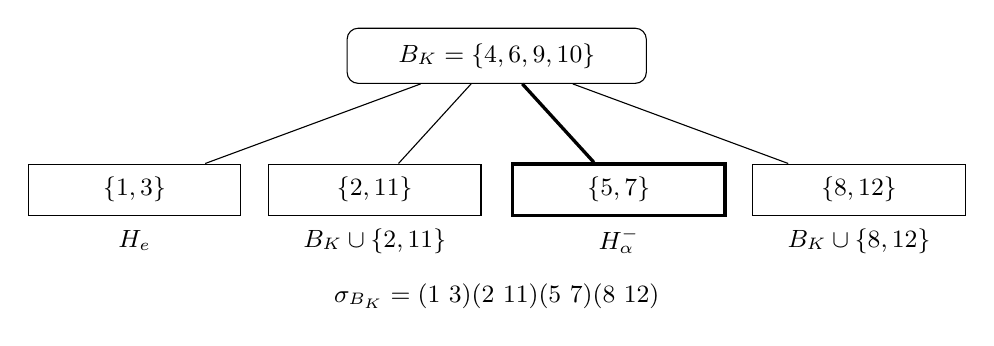
\begin{tikzpicture}[x=1cm,y=1cm, every node/.style={font=\small}]
 \node[draw,rounded corners,minimum width=3.8cm,minimum height=.7cm]
  (b) at (0,0) {$B_K=\{4,6,9,10\}$};
 \node[draw,minimum width=2.7cm,minimum height=.65cm]
  (p1) at (-4.6,-1.7) {$\{1,3\}$};
 \node[draw,minimum width=2.7cm,minimum height=.65cm]
  (p2) at (-1.55,-1.7) {$\{2,11\}$};
 \node[draw,very thick,minimum width=2.7cm,minimum height=.65cm]
  (p3) at (1.55,-1.7) {$\{5,7\}$};
 \node[draw,minimum width=2.7cm,minimum height=.65cm]
  (p4) at (4.6,-1.7) {$\{8,12\}$};
 \draw (b) -- (p1); \draw (b) -- (p2);
 \draw[very thick] (b) -- (p3); \draw (b) -- (p4);
 \node at (-4.6,-2.35) {$H_e$};
 \node at (-1.55,-2.35) {$B_K\cup\{2,11\}$};
 \node at (1.55,-2.35) {$H^-_\alpha$};
 \node at (4.6,-2.35) {$B_K\cup\{8,12\}$};
 \node at (0,-3.05)
  {$\sigma_{B_K}=(1\ 3)(2\ 11)(5\ 7)(8\ 12)$};
\end{tikzpicture}
\caption{L'étoile concrète du drapeau dodécaphasique. Chaque ligne
indique l'union du quadruplet central avec la paire à son extrémité ; la
ligne épaisse signale l'hexade également sélectionnée par les signes
antérieurs à la retenue de $\alpha$. Les quatre paires épuisent les huit
positions extérieures.}
\label{exc:fig-estrella}
\end{figure}

\begin{proposition}[La collection d'étoiles]
\label{exc:m12}
Les $\binom{12}4=495$ permutations $\sigma_B$ préservent $\mathcal H$.
Le groupe qu'elles engendrent est d'ordre $95040$ et est le groupe de Mathieu
$M_{12}$ dans son action sur le petit système de Witt.
\end{proposition}

\begin{proof}
L’affirmation de préservation est une vérification finie sur les
$132$ hexades de \eqref{exc:codigo} : pour chaque quadruplet, on construit
les quatre pétales et on vérifie
$\{\sigma_B(H):H\in\mathcal H\}=\mathcal H$.
La clôture par composition de ces permutations produit $95040$
éléments. Dans l’énumération lexicographique, il suffit d’ajouter successivement
six étoiles qui ne sont pas encore contenues dans le groupe ; les ordres intermédiaires
sont $2,6,18,360,7920,95040$, et les $495$ étoiles appartiennent au groupe
final. L’appendice~\ref{iv:apendice-estrellas} présente les six
permutations et la récurrence finie de clôture. Enfin, on applique la reconnaissance
du groupe des automorphismes de $S(5,6,12)$ comme $M_{12}$, dont l’ordre est
$12\cdot11\cdot10\cdot9\cdot8=95040$.
\end{proof}

Une étoile individuelle engendre un groupe cyclique d'ordre deux. Elle
n'engendre pas à elle seule $M_{12}$, et encore moins le Monstre. L'
existence de $495$ générateurs d'un groupe de permutations ne prouve pas non plus que
chacun soit le transport d'un lacet spécifique du TPK. Cette affirmation
requiert l'application de lacets correspondante ; le résultat établi ici
est l'action d'incidence finie.

\begin{remark}[L'égalité des traces n'identifie pas les opérateurs]
Sur $V_{11}$, une étoile a pour spectre $+1$ avec multiplicité sept
et $-1$ avec multiplicité quatre. Sa trace normalisée est $3/11$.
Un projecteur de rang trois sur le même espace possède également une trace
normalisée $3/11$, mais un spectre $1^3,0^8$. Ils ne sont pas conjugués : leurs
polynômes minimaux et leurs spectres sont différents. L'opérateur d'entrelacement
\eqref{exc:incidencia} transporte des opérateurs définis ; il ne transforme pas
cette coïncidence scalaire en une équivalence d'opérateurs.
\end{remark}

% Recuperación aditiva: comunicados Witt v4--v7, tablas originales y
% RECUPERACION_ESTRELLAS_NONADICA_20260926. La procedencia completa está
% en el mapa editorial; el texto público conserva objetos y pruebas.
\subsection{Trois étoiles régionales et polarisation de leurs complétions}
\label{star27:comparacion}

La construction d'incidence précédente permet de comparer les régions au moyen d'une même opération. Les mots régionaux proviennent de l'émission APP--TRIT--TPK ; leur codage par \(\gamma_{A_W}(w)=(w,wA_W)\) conserve un support dans les douze positions. Le registre \(K\) et la cochaîne antérieure à la retenue ajoutent deux lectures du même état : la position par rapport à la frontière \(729+271\) et l'orientation des emprunts. La comparaison qui suit réunit ces données déjà construites et maintient leur ordre causal.

Les tableaux conservés utilisent également une présentation équivalente.
\par % S27_LAYOUT_PARAGRAPH
Si \(D=\operatorname{diag}(1,-1,-1,-1,-1,-1)\) dans
\(\mathbb F_3\), sa matrice est \(A_{\rm hist}=A_WD\), et
\[
\gamma_{A_{\rm hist}}(w)=\gamma_{A_W}(w)(I_6\oplus D).
\]
Le changement multiplie les coordonnées par des unités et conserve tous les
supports. Par conséquent, les tableaux d'étoiles se transportent
intégralement vers la présentation \(A_W\) utilisée ici.

Écrivons
\[
\begin{aligned}
w_\pi&=010211,&w_e&=201101,&
w_\varphi&=121200,&w_{\rm APP}&=022020,\\
P_\pi&=\{2,4,5,6,7,8,9,10,11\},&
H_e&=\{1,3,4,6,9,10\},\\
H_\varphi&=\{1,2,3,4,7,9\},&
H_{\rm APP}&=\{2,3,5,10,11,12\}.
\end{aligned}
\]
Les quatre ensembles des deuxième et troisième lignes sont les supports
des mots codés correspondants. La cochaîne
\[
s=(7,297,353,-430,-715,-1199,-3,286,-894,-528,380,663)
\]
détermine la partition
\[
H^-_\alpha=\{4,5,6,7,9,10\},\qquad
H^+_\alpha=\{1,2,3,8,11,12\}.
\]
Les signes sont ainsi fixés avant la normalisation décimale.
Pour un quadruplet \(B\), notons
\[
\mu_W(B)=\{H\setminus B:H\in\mathcal H,\ B\subset H\}
\]
l'appariement de son étoile. Une paire est de type \(++\), \(--\) ou \(+-\) selon qu'elle contient zéro, deux ou un point de \(H^-_\alpha\). Sa signature est \(\nu(B)=(n_{++}(B),n_{--}(B),n_{+-}(B))\).

\begin{proposition}[Comparaison des trois intersections régionales]
\label{star27:tres}
Les quadruplets
\[
B_K=H_e\cap P_\pi,\qquad
B_\varphi=H_\varphi\cap P_\pi,\qquad
B_{\rm APP}=H_{\rm APP}\cap P_\pi
\]
ont les douze complétions et les signatures indiquées dans le
tableau~\ref{star27:tabla-tres}.
\end{proposition}

\begin{table}[htbp]
\centering\small
\begin{tabular}{lll}
\toprule
Quadruplet et signature & Paire ajoutée & Hexada resultante\\
\midrule
\(B_K=\{4,6,9,10\}\) & \(\{1,3\}_{++}\) & \(\{1,3,4,6,9,10\}\)\\
\(\nu(B_K)=(3,1,0)\) & \(\{2,11\}_{++}\) & \(\{2,4,6,9,10,11\}\)\\
 & \(\{5,7\}_{--}\) & \(\{4,5,6,7,9,10\}\)\\
 & \(\{8,12\}_{++}\) & \(\{4,6,8,9,10,12\}\)\\
\midrule
\(B_\varphi=\{2,4,7,9\}\) & \(\{1,3\}_{++}\) & \(\{1,2,3,4,7,9\}\)\\
\(\nu(B_\varphi)=(1,0,3)\) & \(\{5,11\}_{+-}\) & \(\{2,4,5,7,9,11\}\)\\
 & \(\{6,12\}_{+-}\) & \(\{2,4,6,7,9,12\}\)\\
 & \(\{8,10\}_{+-}\) & \(\{2,4,7,8,9,10\}\)\\
\midrule
\(B_{\rm APP}=\{2,5,10,11\}\) & \(\{1,4\}_{+-}\) & \(\{1,2,4,5,10,11\}\)\\
\(\nu(B_{\rm APP})=(1,1,2)\) & \(\{3,12\}_{++}\) & \(\{2,3,5,10,11,12\}\)\\
 & \(\{6,7\}_{--}\) & \(\{2,5,6,7,10,11\}\)\\
 & \(\{8,9\}_{+-}\) & \(\{2,5,8,9,10,11\}\)\\
\bottomrule
\end{tabular}
\caption{Les trois étoiles avec la même polarisation de référence.
Chaque ligne conserve le quadruplet, la paire complémentaire et l'hexade complète.}
\label{star27:tabla-tres}
\end{table}

\begin{proof}
On applique \(\gamma_{A_W}\) aux quatre mots régionaux et l'on obtient les supports écrits. Pour chaque quadruplet, on énumère les hexades de \(\mathcal H\) qui le contiennent. La propriété \(\lambda_4=4\) garantit que les quatre complétions du tableau épuisent l'étoile. Enfin, l'intersection de chaque paire avec \(H^-_\alpha\) détermine son signe. Toutes les opérations ont lieu sur le plan combinatoire fini déjà construit.
\end{proof}

Les trois signatures distinguent des fonctions d'incidence précises.
L'étoile de \(B_K\) sépare trois paires positives et une paire négative ; celle
de \(B_\varphi\) contient trois paires mixtes ; celle de \(B_{\rm APP}\)
combine les trois classes. La différence se conserve même lorsque
deux étoiles partagent la paire \(\{1,3\}\).

\begin{figure}[htbp]
\centering
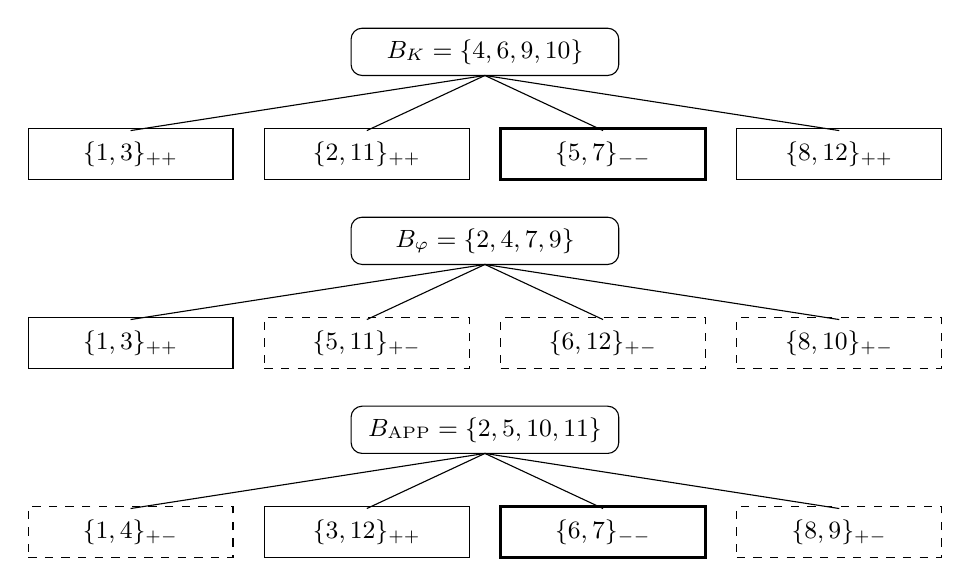
\begin{tikzpicture}[x=1cm,y=1cm,every node/.style={font=\small},
 core/.style={draw,rounded corners,minimum width=3.4cm,minimum height=.6cm},
 petal/.style={draw,minimum width=2.6cm,minimum height=.65cm}]
\foreach \y/\name in {0/{B_K=\{4,6,9,10\}},
 -2.4/{B_\varphi=\{2,4,7,9\}},-4.8/{B_{\rm APP}=\{2,5,10,11\}}}
 {\node[core] at (0,\y) {\(\name\)};
  \foreach \x in {-4.5,-1.5,1.5,4.5}
    {\draw (0,\y-.3)--(\x,\y-1);}}
\node[petal] at (-4.5,-1.3) {\(\{1,3\}_{++}\)};
\node[petal] at (-1.5,-1.3) {\(\{2,11\}_{++}\)};
\node[petal,very thick] at (1.5,-1.3) {\(\{5,7\}_{--}\)};
\node[petal] at (4.5,-1.3) {\(\{8,12\}_{++}\)};
\node[petal] at (-4.5,-3.7) {\(\{1,3\}_{++}\)};
\node[petal,dashed] at (-1.5,-3.7) {\(\{5,11\}_{+-}\)};
\node[petal,dashed] at (1.5,-3.7) {\(\{6,12\}_{+-}\)};
\node[petal,dashed] at (4.5,-3.7) {\(\{8,10\}_{+-}\)};
\node[petal,dashed] at (-4.5,-6.1) {\(\{1,4\}_{+-}\)};
\node[petal] at (-1.5,-6.1) {\(\{3,12\}_{++}\)};
\node[petal,very thick] at (1.5,-6.1) {\(\{6,7\}_{--}\)};
\node[petal,dashed] at (4.5,-6.1) {\(\{8,9\}_{+-}\)};
\end{tikzpicture}
\caption{Comparaison des trois étoiles. Chaque connexion représente
l'union du quadruplet supérieur avec une paire ; les douze hexades
complètes figurent dans le tableau~\ref{star27:tabla-tres}. Le contour
épais signale les paires négatives et le contour discontinu les paires mixtes.
Les connexions représentent l'incidence.}
\label{star27:figura}
\end{figure}

\begin{proposition}[Couplage de la couronne, de l'incidence et du signe]
\label{star27:acoplamiento}
Pour le registre dodécaphasique préalablement construit,
\[
B_K=\{i:K_i\geq729\}=H_e\cap P_\pi=\{4,6,9,10\}.
\]
L'unique hexade \(H\in\mathcal H\) qui satisfait
\(H\cap P_\pi=B_K\) est \(H_e\). De plus,
\[
H^-_\alpha=B_K\sqcup\{5,7\},\qquad
(B_\varphi\setminus B_K)\cap H^-_\alpha=\{7\}.
\]
\end{proposition}

\begin{proof}
Le registre
\(K=(234,543,140,729,659,824,621,58,914,794,146,601)\)
dépasse ou atteint \(729\) précisément aux quatre positions
indiquées. Sa comparaison avec les supports prouve la première
égalité. Une hexade dont l'intersection est \(B_K\) doit appartenir à
l'étoile de \(B_K\) ; parmi ses quatre paires, seule \(\{1,3\}\) est
disjointe de \(P_\pi\). Cela prouve l'unicité relative de \(H_e\).
Le tableau identifie la paire négative \(\{5,7\}\). Enfin,
\(B_\varphi\setminus B_K=\{2,7\}\), et les signes
\(s_2=297>0\), \(s_7=-3<0\) déterminent le pivot \(7\).
\end{proof}

Le quadruplet, le signe et la normalisation conservent des fonctions distinctes. L'incidence fixe la complétion \(H^-_\alpha\) ; le relèvement archimédien de la cochaîne complète utilise en outre les grandeurs, l'ordre positionnel et les retenues déjà démontrés dans la clôture de \(\alpha\). Cette composition explique comment une même généalogie produit une lecture géométrique de frontière et une lecture numérique.

\subsection{Classification polarisée des 495 quadruplets}
\label{star27:clasificacion}

\begin{theorem}[Recensement des signatures et restriction régionale]
\label{star27:censo}
Les \(495=\binom{12}{4}\) quadruplets se répartissent selon le tableau
\ref{star27:tabla-censo}. La dernière colonne compte les hexades
\(H\) avec \(|H\cap P_\pi|=4\), classées selon
\(\nu(H\cap P_\pi)\).
\end{theorem}

\begin{table}[htbp]
\centering
\begin{tabular}{ccc}
\toprule
\(\nu=(n_{++},n_{--},n_{+-})\)&Quadruplets&Hexadas regionales\\
\midrule
\((3,1,0)\)&15&9\\
\((1,3,0)\)&15&0\\
\((2,2,0)\)&45&9\\
\((1,1,2)\)&180&18\\
\((1,0,3)\)&120&18\\
\((0,1,3)\)&120&0\\
\midrule
Total&495&54\\
\bottomrule
\end{tabular}
\caption{Classification complète et restriction au support \(P_\pi\).
Les deux colonnes comptent des objets distincts : quadruplets et hexades.}
\label{star27:tabla-censo}
\end{table}

\begin{proof}
La procédure suivante constitue une énumération exacte du domaine fini. On forme les \(3^6\) mots \(w\), on calcule \((w,wA_W)\) modulo \(3\) et on conserve leurs supports de poids six sans répétition ; on obtient ainsi \(\mathcal H\), avec \(132\) éléments. Pour chaque \(B\in\binom{[12]}4\), on forme \(\mu_W(B)\), on compte les intersections de ses quatre paires avec \(H^-_\alpha\) et on incrémente l'entrée de la signature résultante. Les six compteurs sont \(15,15,45,180,120,120\). Leur somme est \(495\), et chaque quadruplet n'est traité qu'une seule fois. Pour la dernière colonne, on parcourt les \(132\) hexades, on retient les \(54\) dont l'intersection est de taille quatre et on applique à cette intersection la même fonction \(\nu\). Les opérations sont des comparaisons d'ensembles et de l'arithmétique dans \(\mathbb F_3\) ; le certificat reproductible conserve le tableau complet des entrées et des sorties.
\end{proof}

La signature \((3,1,0)\) appartient à quinze quadruplets. La
caractérisation du cadre régional utilise conjointement la couronne
de \(K\), l'intersection \(H_e\cap P_\pi\) et le signe de la
cochaîne, comme l'établit la proposition~\ref{star27:acoplamiento}.

\subsection{Rigidité du cadre ordonné de quatre supports}
\label{star27:rigidez}

Soit \(G_W=\langle\sigma_B:|B|=4\rangle\), déjà calculé dans la
proposition~\ref{exc:m12}. Pour une collection ordonnée de supports,
nous définissons
\[
\operatorname{Stab}_{G_W}(S_1,\ldots,S_r)
=\{g\in G_W:g(S_j)=S_j\ \text{pour tout }j\}.
\]
Chaque support est conservé individuellement ; les permutations internes
de ses points restent permises.

\begin{theorem}[Rigidité conjointe des quatre incidences]
\label{star27:marco}
Les stabilisateurs ont les ordres suivants :
\[
\begin{array}{l|r}
\text{données préservées}&\text{ordre}\\ \hline
H^-_\alpha&720\\
H^-_\alpha,\ 6&120\\
B_K&192\\
B_K,H^-_\alpha&48\\
B_K,H^-_\alpha,H_e&16\\
H^-_\alpha,H_e,H_\varphi&2\\
H^-_\alpha,H_e,H_\varphi,H_{\rm APP}&1
\end{array}
\]
Dans la deuxième ligne, le point \(6\) est également conservé.
En particulier,
\[
\operatorname{Stab}_{G_W}
(H^-_\alpha,H_e,H_\varphi,H_{\rm APP})=\{\operatorname{id}\}.
\]
\end{theorem}

\begin{proof}
On utilise la clôture par composition des six permutations
explicites de la proposition~\ref{exc:m12}. Sur ses \(95040\)
éléments, on évalue les prédicats \(g(S_j)=S_j\), conjointement avec
\(g(6)=6\) lorsque cela s'applique. Les sommes des indicatrices de
ces prédicats donnent, respectivement,
\(720,120,192,48,16,2,1\). L'identité satisfait toutes les
conditions ; le dernier cardinal prouve qu'elle est l'unique élément.
L'algorithme de clôture s'arrête par stabilité de l'ensemble,
et les filtres de stabilisation s'appliquent ensuite au groupe complet.
\end{proof}

Le tableau compare sept configurations marquées. Deux chaînes
d'inclusions utiles sont celles déterminées par
\((B_K)\), \((B_K,H^-_\alpha)\), \((B_K,H^-_\alpha,H_e)\),
et par
\((H^-_\alpha)\), \((H^-_\alpha,H_e,H_\varphi)\),
\((H^-_\alpha,H_e,H_\varphi,H_{\rm APP})\).
La rigidité finale exprime que le cadre régional ordonné fixe
complètement la liberté résiduelle au sein de \(G_W\). Son domaine est
l'action sur les douze positions ; le transport ultérieur vers les
réseaux et les algèbres conserve les applications propres à ces réalisations.

\subsection{Topologie finie de l'incidence et conservation de son domaine}
\label{star27:topologia}

Le complexe simplicial engendré par les \(132\) hexades a pour vecteur
de faces
\[
(f_0,f_1,f_2,f_3,f_4,f_5)=(12,66,220,495,792,132)
\]
et la caractéristique d'Euler \(\chi=12-66+220-495+792-132=331\). En effet, chaque ensemble de cinq points possède une extension hexadique unique ; tout sous-ensemble de cardinal inférieur appartient à l'un de ces ensembles, et les faces maximales sont les hexades.

Le graphe biparti entre quadruplets et hexades possède
\[
|V|=495+132=627,\qquad |E|=495\cdot4=132\cdot15=1980.
\]
Il est connexe. Soient \(H\) et \(H_*\) deux hexades distinctes ; leur
intersection comporte au plus quatre points, car l'extension
d'un quintuplet est unique. Choisissons un quadruplet \(B\subset H\)
qui contienne \(H\cap H_*\), et un point \(p\in H_*\setminus H\).
L'unique extension \(H'\) de \(B\cup\{p\}\) est reliée à
\(H\) par le chemin biparti \(H-B-H'\) et satisfait
\(|H'\cap H_*|>|H\cap H_*|\). En répétant l'opération, on
atteint \(H_*\) ; contenir cinq de ses points impose déjà
l'égalité. Tout quadruplet possède quatre hexades incidentes, de
sorte qu'il appartient également à cette composante unique.
Son premier nombre de Betti est donc
\[
\beta_1=|E|-|V|+1=1354.
\]
Le parcours exhaustif de l'incidence vérifie aussi la
connexité. Pour les paires non ordonnées d'hexades distinctes, le recensement
des tailles d'intersection est
\[
\begin{array}{c|rrrr}
|H\cap H'|&0&2&3&4\\ \hline
\#\{H,H'\}&66&2970&2640&2970 .
\end{array}
\]
La somme \(8646=\binom{132}{2}\) couvre toutes les paires.

Ces invariants décrivent le complexe et son graphe d'incidence.
Le micrographe de raccordements \(U_6=A|B\) conserve séparément ses
\(96\) sommets, \(234\) arêtes, six composantes et
\(\beta_1=234-96+6=144\). De même, la composition des
\(\sigma_B\) agit sur des positions d'incidence, tandis que
\(\Gamma_9\) transporte l'état TPK à mémoire. Cette précision
permet de relier les lectures au moyen de leurs applications effectives et de
conserver, à chaque niveau, les données utilisées par l'opération.


\subsection{Le résidu binaire et les cinq régions de \texorpdfstring{$\pi$}{pi}}
\label{exc:cinco-regiones}

La reconnaissance suivante utilise le code de Golay binaire
étendu $G_{24}$, de paramètres $[24,12,8]_2$. Ses poids sont
$0,8,12,16,24$, et les supports de poids huit forment le plan
$S(5,8,24)$. Nous fixons une dodécade $D$, support d'un mot de poids
douze. Cette donnée et l'isomorphisme d'incidence qui sera déclaré
ci-après appartiennent à la coordinatisation de réalisation ; ils ne sont pas utilisés pour
engendrer ni sélectionner les décimales de $\pi$.

\begin{proposition}[Résidu d'une dodécade et élévation d'hexades]
\label{exc:residuo-binario}
L'ensemble
\[
 \mathcal H(D)=
 \{O\cap D: O\text{ est une octade},\ |O\cap D|=6\}
\]
est un système $S(5,6,12)$ sur $D$. Chacune de ses hexades a une unique élévation en une octade. Pour tout quadruplet $B\subset D$, les cinq octades qui le contiennent se répartissent en quatre élévations résiduelles et une unique octade $O_B^\perp$ avec $O_B^\perp\cap D=B$.
\end{proposition}

\begin{proof}
Un quintuplet $A\subset D$ appartient à une unique octade $O$. Si
$j=|O\cap D|$, le mot binaire somme de $O$ et $D$ a pour poids
$20-2j$. Parmi les poids permis, et avec $0\leq j\leq8$, seuls
$j=2,4,6$ sont possibles. Comme $A\subset O\cap D$, on a $j\geq5$
et donc $j=6$. Cela donne l'existence et l'unicité de l'hexade
résiduelle, ainsi que l'unicité de son élévation en choisissant cinq de ses
points. D'autre part,
\[
 \lambda_4(S(5,8,24))=\frac{\binom{20}1}{\binom41}=5,
 \qquad
 \lambda_4(S(5,6,12))=4.
\]
Les quatre hexades résiduelles sur $B$ donnent quatre octades distinctes. La cinquième ne peut pas couper $D$ en six points, car elle serait une autre hexade résiduelle ; puisqu'elle contient $B$, son intersection est de taille quatre et coïncide avec $B$.
\end{proof}

Une coordinatisation $\ell:[12]\to D$ qui préserve les hexades identifie
$\mathcal H$ à $\mathcal H(D)$. Son existence est la reconnaissance
du plan déjà construit comme le petit plan de Witt ; un choix
précis de $\ell$ fixe le réétiquetage. Le relèvement
\[
 \iota_D:\mathcal H\longrightarrow
       \{\text{octades de }G_{24}\},
 \qquad H\longmapsto O\text{ tel que }O\cap D=\ell(H),
\]
est injective parce que l'intersection avec $D$ redonne $\ell(H)$. Cette injectivité a pour domaine les hexades, et non le registre $K$.

La relation avec les cinq régions de $\pi$ conserve des données plus riches
que le nombre cinq. Les émissions et leurs signatures sont :
\begin{center}
\small
\begin{tabular}{@{}crll@{}}
\toprule
Région & Multiplicité & Émission $U_6$ & Signature \\
\midrule
$\perp$ & $432$ & $(501,614,498,169,272,272)$ & $555555$ \\
$++_1$ & $144$ & $(810,923,870,169,272,272)$ & $339555$ \\
$++_2$ & $144$ & $(810,983,810,169,272,272)$ & $393555$ \\
$++_3$ & $144$ & $(870,923,810,169,272,272)$ & $933555$ \\
$--$ & $144$ & $(870,923,810,418,674,521)$ & $933717$ \\
\bottomrule
\end{tabular}
\end{center}
Dans chaque bloc décimal de trois chiffres, la signature utilise la différence
modulaire des deux premiers chiffres. Les cinq émissions ont le
même mot tritique visible $w_\pi=010211$, mais pas la même
généalogie régionale. Les trois régions positives conservent la queue
$169|272|272$ ; la région négative la remplace par $418|674|521$ ;
la région transversale a une signature constante et une multiplicité supérieure.

L'extension marquée de la coordinatisation régionale envoie la région transversale
sur $O_{\ell(B_K)}^\perp$, la région négative sur $\iota_D(H^-_\alpha)$ et les
trois régions positives sur les trois autres relèvements de l'étoile. Ainsi se
réalise la partition $4+1$ des cinq octades sur $\ell(B_K)$.
La correspondance individuelle entre les trois noms positifs et
les trois pétales restants exige un ordre de coordinatisation ; l'incidence ne la détermine
pas sans cette donnée. L'énoncé précis est donc une
correspondance marquée des régions, compatible avec leurs rôles et avec
le drapeau, et non une bijection canonique déduite du cardinal cinq.

L'identité $432+4\cdot144=1008$ conserve les multiplicités
régionales. On a aussi $1008=36\cdot28$, et une octade possède
$\binom82=28$ paires. Ces égalités sont des contrôles arithmétiques du
catalogue, et non des substituts à l'application $\iota_D$ ni à la coordinatisation régionale.

\subsubsection{Représentation pentadique de la microfibre et de son incidence}
\label{pi-estrella:desarrollo}

La disposition des cinq régions permet de visualiser simultanément
l'unité du quotient ternaire et la différenciation conservée par le
catalogue. L'application pertinente est la restriction
\[
 \Psi\big|_{\mathscr R_\pi^{\rm micro}}:
 \mathscr R_\pi^{\rm micro}\longrightarrow\{010211\},
 \qquad \Psi(U)=(-U)\bmod3.
\]
Ses cinq antécédents sont les vecteurs \(U_6\) du tableau précédent.
La figure \ref{pi-estrella:figura} retrouve leur organisation radiale,
en conservant l’ordre du système de coordonnées, les signatures et les multiplicités du
catalogue de la section~\ref{exc:cinco-regiones}, calculable
à l’aide de la récurrence et des signatures de l’appendice~\ref{iv:apendice-firmas}.

% Orden de carta y datos recuperados de fig_cinco_regiones_pi.tex.
\begin{figure}[H]
\centering
\begin{tikzpicture}[x=1cm,y=1cm,font=\small,>=Latex]
 \coordinate (a) at (90:2.2);
 \coordinate (b) at (18:2.2);
 \coordinate (c) at (-54:2.2);
 \coordinate (d) at (-126:2.2);
 \coordinate (e) at (162:2.2);
 \draw[black!35,line width=.45pt]
    (a)--(c)--(e)--(b)--(d)--cycle;
 \node[draw,fill=white,circle,minimum size=1.6cm,align=center,
    inner sep=3pt] (z) at (0,0) {$w_\pi$\\$010211$};
 \foreach \v in {a,b,c,d,e}{
    \fill (\v) circle (2pt);
    \draw[->,line width=.6pt] (\v)--(z);
 }
 \node[above=3mm,align=center] at (a)
   {$U_\pi^\perp$\\$555555$\\multiplicidad $432$};
 \node[right=3mm,align=left] at (b)
   {$U_{\pi,1}^{++}$\\$339555$\\multiplicidad $144$};
 \node[below right=2mm and 1mm,align=left] at (c)
   {$U_{\pi,2}^{++}$\\$393555$\\multiplicidad $144$};
 \node[below left=2mm and 1mm,align=right] at (d)
   {$U_{\pi,3}^{++}$\\$933555$\\multiplicidad $144$};
 \node[left=3mm,align=right] at (e)
   {$U_\pi^{--}$\\$933717$\\multiplicidad $144$};
 \node[align=center,font=\footnotesize] at (0,-3.55)
   {$1_\perp+3_{++}+1_{--}$\qquad $432+4\cdot144=1008$};
\end{tikzpicture}
\caption{Les cinq régions de \(\pi\) en disposition pentadique.
Chaque position conserve sa signature multiplicative et sa multiplicité ;
les flèches radiales représentent la projection commune
\(\Psi(U)=010211\). Le contour étoilé organise les cinq
positions de la coordinatisation. Leur réalisation dans les cinq octades de Witt
s'effectue par l'alignement régional et la décomposition
\(4+1\) du texte.}
\label{pi-estrella:figura}
\end{figure}


La projection sur le centre identifie les cinq images ternaires ; le
registre des positions extérieures retient l'information régionale
qui rend possible la réalisation d'incidence. La distribution
\(1_\perp+3_{++}+1_{--}\) spécifie une région transversale, trois
régions positives et une négative. Leurs poids normalisés sont
\(3/7\) et \(1/7\) pour chacune des quatre autres : la
multiplicité transversale est triple, alors même que les cinq images par
\(\Psi\) coïncident.

\Needspace{11\baselineskip}
Le lien avec l'étoile de Witt se formule au moyen du drapeau
\(B_K\subset H^-_\alpha\), de l'alignement \(\ell\) et du
relèvement \(\iota_D\) déjà construits. Les cinq positions régionales
se réalisent dans les cinq octades sur \(\ell(B_K)\) :
\[
\begin{aligned}
 U_\pi^\perp&\longmapsto O^\perp_{\ell(B_K)},\\
 U_\pi^{--}&\longmapsto\iota_D(H^-_\alpha),\\
 \{U_{\pi,1}^{++},U_{\pi,2}^{++},U_{\pi,3}^{++}\}
 &\longmapsto
 \{\iota_D(B_K\cup P):P\in\mathcal P_+\},\\
 \mathcal P_+&=\bigl\{\{1,3\},\{2,11\},\{8,12\}\bigr\}.
\end{aligned}
\]
L'assignation des trois positions positives aux trois paires
s'effectue dans une coordinatisation ordonnée. La ligne transversale et la ligne négative
sont distinguées par leurs prédicats régionaux et par le drapeau.

Les deux figures s'articulent ainsi : la figure
\ref{exc:fig-estrella} montre les quatre hexades du petit plan
de Witt sur \(B_K\) ; la figure \ref{pi-estrella:figura} montre
les cinq régions qui, sous l'alignement, occupent les quatre octades
résiduelles et l'octade transversale du plan binaire. La loi
\(4+1\), démontrée dans la proposition
\ref{exc:residuo-binario}, spécifie le changement d'incidence. Dans cette
composition, \(K\) détermine la tétrade marquée et la signature de
\(\alpha\) distingue l'une de ses hexades. Les régions conservent,
outre leur valeur ternaire commune, la structure nécessaire à ce
transport vers la réalisation exceptionnelle.


\subsection{Du code ternaire au réseau de Niemeier}
\label{exc:niemeier}

Le passage à la dimension vingt-quatre ne nécessite pas de parcourir d'abord le
code binaire. Il s'effectue directement à partir de $C_W$ par recollement des
discriminants. On distingue ainsi deux prolongations compatibles :
l'une conserve le résidu $W_{12}\subset W_{24}$ ; l'autre construit le
réseau sur lequel sera réalisée l'algèbre d'opérateurs de vertex.

Soit $A_2=\mathbb Z a_1\oplus\mathbb Z a_2$ de matrice de Gram
\[
 \begin{pmatrix}2&-1\\-1&2\end{pmatrix},
 \qquad \rho=a_1+a_2,\qquad \rho^2=2.
\]
Nous représentons les trois classes de $A_2^*/A_2$ par
\[
 \varpi_0=0,\qquad
 \varpi_1=\frac{2a_1+a_2}{3},\qquad
 \varpi_2=\frac{a_1+2a_2}{3}.
\]
L'application $j\mapsto\varpi_j+A_2$ identifie additivement
$\mathbb F_3$ à ce discriminant. Pour $c\in C_W$, nous écrivons
$\phi(c)=(\varpi_{c_1},\ldots,\varpi_{c_{12}})$ et définissons
\begin{equation}
 N(C_W)=\bigcup_{c\in C_W}\bigl(A_2^{12}+\phi(c)\bigr).
 \label{exc:niemeier-def}
\end{equation}

\begin{theorem}[Pegado ternario]
\label{exc:niemeier-teorema}
L'objet \eqref{exc:niemeier-def} est un réseau positif, pair et
unimodulaire de rang $24$. Son système de racines est exactement
$A_2^{12}$ ; il est donc reconnu comme le réseau de Niemeier ayant
ce système de racines.
\end{theorem}

\begin{proof}
La linéarité du code rend l'union de classes stable par addition. L'auto-orthogonalité annule l'accouplement discriminant : celui-ci est un multiple de $c\cdot d/3$ modulo $\mathbb Z$. Le réseau est donc entier. La norme d'une classe de recollement est $2\operatorname{wt}(c)/3$ modulo $2\mathbb Z$. Les poids de \eqref{exc:enumerador} sont des multiples de trois, de sorte qu'il est pair.

L'indice de $A_2^{12}$ dans $N(C_W)$ est $|C_W|=3^6$. En conséquence,
\[
 \det N(C_W)=\frac{3^{12}}{(3^6)^2}=1.
\]
La positivité procède de la somme orthogonale des douze métriques $A_2$.
Dans une classe non nulle de $A_2^*/A_2$, la norme minimale est $2/3$ ;
tout mot non nul possède au moins six positions non nulles.
Par conséquent, un vecteur d'une classe de recollement non triviale a une norme
au moins égale à $6\cdot2/3=4$. Aucune racine de norme deux n'apparaît hors de
$A_2^{12}$. À l'intérieur de celui-ci, les racines sont précisément celles de ses
douze composantes.
\end{proof}

\subsection{Sélection par incidence du voisin unimodulaire sans racines}
\label{exc:leech}

\paragraph{De l'origine incidencielle à la modification réticulaire.}
\label{inc-ampl-reticulo}
Le drapeau marqué détermine une position au moyen d'une opération
ensembliste équivariante :
\[
 o_*=(H_e\cap H_\varphi)
       \setminus(H^-_\alpha\cup H_{\rm APP})=\{1\}.
\]
Sa fonction consiste à distinguer une composante parmi les douze qui
interviennent dans la réalisation réticulaire. Le code ternaire complet
agit comme code de recollement dans le module discriminant
$(A_2^*/A_2)^{12}$. Sa préimage définit $N(C_W)$, et
l'autodualité, les poids et la distance du code se traduisent,
respectivement, en propriétés d'intégralité et de déterminant, de parité
et en bornes de norme des classes de recollement. L'information symbolique
du code remplit ici une fonction que le support isolé ne remplit plus.

La métrique $A_2$ et la chambre radiale positive sont fixées dans le développement
réticulaire. À l'intérieur de cette chambre, la congruence nécessaire pour un voisin
pair d'indice trois possède douze réalisations de norme minimale $54$,
permutées par le changement de composante distinguée. L'origine $o_*$
sélectionne
\[
 v_\alpha=4\rho_1+\rho_2+\cdots+\rho_{12},\qquad
 v_\alpha^2=2(4^2+11)=54.
\]
Le coefficient $4$ appartient à cette solution de la congruence dans la
chambre déclarée. L'indice $\alpha$ enregistre la provenance
incidencielle de la sélection : son contenu est le repère qui est intervenu dans
la clôture et qui individualise à présent une direction réticulaire.

L'appariement avec $v_\alpha$ détermine le sous-réseau
$N_{\alpha,0}$ d'indice trois, et l'adjonction de la classe
$v_\alpha/3$ produit le voisin $N_\alpha$ de
\eqref{exc:vecino}. Cette modification conserve le rang et rétablit
l'unimodularité et la parité ; la sélection par congruence élimine les racines
antérieures, et les bornes locales excluent les racines dans les nouvelles classes.
L'identification à Leech intervient après ces vérifications. La
réalisation binaire des cinq régions et cette construction réticulaire
sont deux prolongements du repère commun : la seconde reçoit directement
le code ternaire comme donnée de recollement.



L'étiquette $o_*=1$ du drapeau se réalise maintenant comme l'une des
douze composantes $A_2$. Cette opération déclare la métrique précédente et
la chambre radiale positive
\[
 v(a)=\sum_{i=1}^{12}a_i\rho_i,
 \qquad a_i=1+3b_i,\quad b_i\in\mathbb Z_{\geq0}.
\]
L'exigence de parité du voisin d'indice trois est $v(a)^2\equiv0\pmod{18}$. Puisque
\[
 v(a)^2=2\sum_i(1+3b_i)^2,
\]
cette congruence équivaut à $\sum_i b_i\equiv1\pmod3$. La plus petite
valeur de la norme dans la chambre s'obtient avec un unique $b_i=1$ et
tous les autres nuls ; elle vaut $54$. L'origine marquée sélectionne
\begin{equation}
 v_\alpha=4\rho_1+\rho_2+\cdots+\rho_{12},
 \qquad v_\alpha^2=54.
 \label{exc:vector}
\end{equation}
Le mot ``plus petit'' se rapporte à cette chambre positive. Il n'affirme pas la minimalité dans toute la classe résiduelle : le vecteur $(a_1-2a_2,\rho,\ldots,\rho)$ représente la même classe modulo trois et a pour norme $14+11\cdot2=36$. La restriction de chambre fait partie des données de la construction, et n'est pas une conclusion que l'on puisse omettre.

Soit $N=N(C_W)$. Nous définissons
\begin{equation}
 N_{\alpha,0}=\{x\in N:\langle x,v_\alpha\rangle\equiv0\pmod3\},
 \qquad
 N_\alpha=N_{\alpha,0}+\mathbb Z\frac{v_\alpha}{3}.
 \label{exc:vecino}
\end{equation}

\begin{theorem}[Voisin de Leech déterminé par le drapeau marqué]
\label{exc:teorema-leech}
Avec la métrique et la chambre déclarées, $N_\alpha$ est un réseau
positif, pair et unimodulaire de rang $24$, sans vecteurs de norme deux.
D'après le théorème de classification correspondant, il est isométrique au
réseau de Leech $\Lambda_{24}$.
\end{theorem}

\begin{proof}
Le caractère $x\mapsto\langle x,v_\alpha\rangle\bmod3$ est non nul :
une racine simple d'une composante s'apparie avec $a_i\rho_i$ en
$a_i\equiv1\pmod3$. Par conséquent, $[N:N_{\alpha,0}]=3$ et
$\det N_{\alpha,0}=9$. De plus,
$v_\alpha/3\in N_{\alpha,0}^*$ et $v_\alpha\in N_{\alpha,0}$.
Si $v_\alpha/3$ appartenait à $N$, l'intégralité de $N$ rendrait
tous les appariements avec $v_\alpha$ divisibles par trois,
ce qui contredirait le caractère non nul. La classe de $v_\alpha/3$ est
donc d'ordre trois. On en déduit
\[
 [N_\alpha:N_{\alpha,0}]=3,
 \qquad \det N_\alpha=9/3^2=1.
\]
L'extension est entière, et pour $x\in N_{\alpha,0}$,
\[
 \left(x+m\frac{v_\alpha}{3}\right)^2
   =x^2+2m\frac{\langle x,v_\alpha\rangle}{3}+6m^2
   \in2\mathbb Z.
\]
Elle est donc paire.

Il reste à exclure les racines, ce qui est l'étape décisive. Les racines de $N$ appartiennent à $A_2^{12}$. Leurs accouplements avec $v_\alpha$ sont congrus à $\pm1$ ou à $\pm2$ modulo trois ; aucune n'appartient à $N_{\alpha,0}$. Pour les deux autres classes du voisin, chaque composante appartient à l'une des classes locales
\[
 A_2+\varpi_j\pm\rho/3,\qquad j=0,1,2.
\]
Comme $4\rho/3\equiv\rho/3\pmod{A_2}$, cette description vaut
également dans la composante distinguée. En écrivant un vecteur local
sous la forme $(u a_1+v a_2)/3$, sa norme est
$2(u^2-uv+v^2)/9$. Les six classes précédentes ont des résidus non
nuls et un minimum $2/9$ : les représentants de forme quadratique minimale
sont $(\pm1,0),(0,\pm1),(1,1),(-1,-1)$ dans les résidus appropriés.
Un vecteur d'une classe nouvelle a donc une norme au moins égale à
$12\cdot2/9=8/3>2$. Aucune des trois classes ne contient de racines.
La classification des réseaux pairs unimodulaires positifs de
rang vingt-quatre identifie l'unique cas sans racines à
$\Lambda_{24}$.
\end{proof}

L'argument ne reconnaît pas Leech par une coïncidence de dimension.
Il construit le recollement, prouve l'intégralité, la parité et le déterminant, et
élimine les racines au moyen d'une borne locale. Ce n'est qu'ensuite qu'il applique le
théorème de classification. La dépendance à l'égard de $\alpha$ est conservée dans
le drapeau qui sélectionne $o_*$ et dans le vecteur \eqref{exc:vector} ;
on ne transforme pas la valeur scalaire de la constante en une longueur du
réseau.

\subsection{L'algèbre d'opérateurs de vertex et le Monstre}
\label{exc:voa}

Soit $\Lambda=N_\alpha$, déjà reconnu comme le réseau de Leech. L'étape suivante utilise son réseau entier, et non un développement décimal. La construction de l'algèbre d'opérateurs de vertex de réseau s'écrit
\[
 V_\Lambda=M(1)\otimes\mathbb C_\varepsilon[\Lambda].
\]
Ici, $M(1)$ est l'espace des oscillateurs de Heisenberg en rang vingt-quatre ; $\mathbb C_\varepsilon[\Lambda]$ est l'algèbre de groupe tordue par le cocycle de l'extension centrale du réseau. Le cocycle et le relèvement des isométries font partie de la construction : une somme vectorielle nue ne détermine pas les produits de vertex.

La négation $\lambda\mapsto-\lambda$ admet le relèvement standard
$\theta$. Avec son module tordu et le choix de parité compatible,
la construction de Frenkel--Lepowsky--Meurman produit
\begin{equation}
 V^\natural_{\rm HMT}
   =V_\Lambda^+\oplus(V_\Lambda^T)^+.
 \label{exc:flm}
\end{equation}
Le signe $+$ désigne la partie paire de l'action relevée. L'expression
inclut le produit de vertex de l'orbifold ; elle ne se limite pas à une somme
d'espaces gradués.

\begin{theorem}[Prolongement jusqu'au module Moonshine]
\label{exc:moonshine}
L'algèbre \eqref{exc:flm}, construite sur le voisin
\eqref{exc:vecino}, est une réalisation de l'algèbre Moonshine
$V^\natural$. Elle a une charge centrale $24$, une composante de poids un nulle
et un groupe d'automorphismes isomorphe au Monstre $\mathbb M$. Son caractère
gradué est
\begin{equation}
 \operatorname{Tr}_{V^\natural_{\rm HMT}}q^{L_0-1}
   =J(\tau)=j(\tau)-744
   =q^{-1}+196884q+21493760q^2+\cdots,
 \qquad q=e^{2\pi i\tau}.
 \label{exc:j}
\end{equation}
\end{theorem}

\begin{proof}
Le théorème \ref{exc:teorema-leech} vérifie les hypothèses sur le réseau :
positivité, parité, unimodularité, rang vingt-quatre et absence de
racines. On applique alors la construction et le théorème de
Frenkel--Lepowsky--Meurman pour le réseau de Leech. Ceux-ci identifient
l'orbifold à $V^\natural$, établissent son caractère et son groupe d'
automorphismes. La composition du drapeau, du voisin et du foncteur
de construction de VOA donne la réalisation indiquée ici. Le groupe ne se déduit
pas du coefficient $196884$.
\end{proof}

Le théorème utilisé est une reconnaissance classique ultérieure dont les hypothèses sont vérifiées, et non une nouvelle démonstration dans cet article de la construction FLM \cite{flm}. En outre, la notation $q=e^{2\pi i\tau}$ est la variable conventionnelle de Fourier employée pour reconnaître le caractère. Elle n'introduit ni $\pi$ ni $e$ comme entrées du générateur coinductif qui les a déjà déterminés.

Une partie du mécanisme de trace peut être observée avant l'orbifold.
Seul le vecteur nul du réseau est fixé par la négation ; chaque
oscillateur contribue avec un signe alterné. D'où
\[
 \operatorname{Tr}_{V_\Lambda}\theta q^{L_0-1}
   =t_2(\tau)
   :=q^{-1}\prod_{n\geq1}(1+q^n)^{-24}.
\]
Cette trace dans l'algèbre de réseau ne doit pas être confondue avec le
caractère sans insertion de $V^\natural$. Elle n'identifie pas non plus à elle
seule une classe de conjugaison du Monstre : l'espace, l'insertion
et le relèvement doivent être spécifiés avant de comparer les fonctions.

\paragraph{Graduation, unité et automorphismes.}
\label{inc-ampl-automorfismos}
La construction de Frenkel--Lepowsky--Meurman s'applique au réseau
$N_\alpha$ une fois ses propriétés vérifiées. Elle incorpore l'espace
des oscillateurs, l'extension centrale du réseau, le produit de vertex
et le secteur tordu par le relèvement de la négation. Le résultat est
l'algèbre $V^\natural_{\rm HMT}$ de \eqref{exc:flm}, dont le groupe
d'automorphismes est isomorphe au Monstre. Son domaine d'action est ainsi
fixé par une structure algébrique munie d'une graduation et d'un produit. Le théorème
de Moonshine de Borcherds détermine ensuite les traces graduées
avec insertion de ces automorphismes \cite{flm,borcherds}.

L'unité acquiert à ce niveau une réalisation précise : la composante
de poids zéro est la droite du vide et fournit le coefficient $1$ de
$q^{-1}$ dans le caractère gradué. Au niveau cylindrique, les
applications de raffinement conservent la fonction constante par
précomposition. Chaque assertion de conservation possède donc son
objet et son application. Le développement des preuves rend visible cette
continuité de construction, depuis les opérations arithmétiques et la
mémoire jusqu'à l'incidence, à la métrique et aux produits de vertex.

Cette articulation situe $K$ et la clôture de $\alpha$ dans l’argument
principal. $K$ conserve réversiblement une coordonnée entière de
l’histoire ; la normalisation de $\alpha$ compose les registres régionaux
avec cette coordonnée ; la configuration signée détermine un drapeau ; et
le drapeau marqué sélectionne la modification réticulaire sur laquelle
Moonshine est réalisé. La proposition~\ref{exc:selector-bandera},
le lemme~\ref{exc:origen} et les théorèmes~\ref{exc:teorema-leech}
et~\ref{exc:moonshine} établissent ces étapes. Les équivalences
réversibles, les quotients d’information et les réalisations qui ajoutent
une métrique ou une structure algébrique conservent ainsi leurs domaines respectifs.
La relation entre structure, équation et valeur s’exprime par ces
applications, avec l’attribution et la portée de chaque résultat.


% Incorporación aditiva para el Artículo I; no modifica la fuente anterior.
% RESULTADO_RECUPERADO: integral, capítulo 22, propietario extenso
% colaboracion/partes_i_ii/source/base_residencias/
% capitulo_22_c20_lineas_2613_3270.tex, líneas 176--576.
% Equivalencia 2/3: public/residencias/capitulo_22_voa_leech_moonshine.tex,
% líneas 55--127. Orden dos y Fricke: hmt/15d_voa_moonshine_orden_dos_rev11.tex.
% Prerrequisitos residentes en I: código C_W, matriz A_W, N(A_2^12),
% origen o_*, vector v_alpha de norma54, N_alpha reconocido como Leech,
% VOA reticular y presentación FLM de las secciones precedentes.
% Bibliografía nueva: chenlamshimakura2016, abelamyamada2017,
% kmconwaynorton1979 (bibitems listos para incorporar al final de este archivo).

\subsection{Orientation ternaire du voisin de Leech}
\label{km:orden-tres-reticular}

La présentation d’ordre deux construite précédemment utilise la négation
du réseau de Leech. Le même réseau, obtenu à partir de l’incidence marquée
par \(K\) et par le support dodécaphasique de \(\alpha\), admet une seconde
présentation compatible avec le caractère ternaire de la construction.
Pour expliciter cette continuité, on conserve le recollement, on construit
son isométrie d’ordre trois et on vérifie qu’elle préserve le voisin déjà
sélectionné. Cette étape n’exige de modifier ni \(K\), ni sa lecture rationnelle ni
la définition préalable de \(\alpha\). La proposition
\ref{km:estabilidad-vecino} vérifie l’isométrie réticulaire ; la proposition
\ref{km:traza-tipo} et le théorème~\ref{km:moonshine-tres} précisent la construction
d’ordre trois et les hypothèses des reconnaissances classiques utilisées.

Nous travaillons dans la base des racines simples de chaque facteur \(A_2\), avec
\begin{equation}
 B_2=\begin{pmatrix}2&-1\\-1&2\end{pmatrix},\qquad
 \mathsf C=\begin{pmatrix}0&-1\\1&-1\end{pmatrix},\qquad
 \mathsf R=\begin{pmatrix}0&1\\1&0\end{pmatrix},\qquad
 \rho=\begin{pmatrix}1\\1\end{pmatrix}.
 \label{km:coxeter-reflexion}
\end{equation}
La multiplication donne
\[
 \mathsf C^3=I_2,\quad
 \mathsf C^2+\mathsf C+I_2=0,\quad
 \mathsf C^{\mathsf T}B_2\mathsf C=B_2,\quad
 \mathsf R\mathsf C\mathsf R=\mathsf C^{-1},\quad
 \mathsf R^{\mathsf T}B_2\mathsf R=B_2.
\]
Ces identités fixent aussi bien la métrique que l'orientation de l'action. Dans le discriminant \(A_2^*/A_2\cong\mathbb F_3\), nous prenons pour générateur la classe de \(\varpi=(2,1)^{\mathsf T}/3\). On a \(\mathsf C\varpi-\varpi=(-1,0)^{\mathsf T}\), de sorte que \(\mathsf C\) agit trivialement sur le discriminant ; la réflexion \(\mathsf R\) change son signe.

La matrice de Paley--Witt déjà construite produit un élément de support
complet par l'opération suivante :
\begin{equation}
 \begin{gathered}
 q_*=(1,1,1,1,1,1),\qquad q_*A_W=(2,1,1,1,1,1),\\
 c_*=(q_*,q_*A_W)
 =(1,1,1,1,1,1,2,1,1,1,1,1)\in C_W.
 \end{gathered}
 \label{km:palabra-total}
\end{equation}
Chaque coordonnée de \(c_*\) est non nulle. Pour les douze positions,
nous définissons les cadres et l'isométrie
\begin{equation}
 P_b(c_*)=
 \begin{cases}\mathsf R,&(c_*)_b=1,\\I_2,&(c_*)_b=2,\end{cases}
 \qquad
 g_c=\bigoplus_{b=1}^{12}P_b(c_*)\mathsf C P_b(c_*)^{-1}.
 \label{km:isometria-ternaria}
\end{equation}
Le symbole \(P_b(c_*)\) désigne ici un repère inversible d’un facteur
\(A_2\), non le projecteur sur l’isotype tridimensionnel \(P_3\)
de la section~\ref{exc:k-direccion}.

\begin{proposition}[Isométrie d'ordre trois sur le voisin marqué]
\label{km:estabilidad-vecino}
L'opérateur \(g_c\) est une isométrie d'ordre trois sans vecteurs fixes non nuls. Il préserve le réseau de Niemeier \(N=N(C_W)\) et le voisin \(N_\alpha\) construit dans \eqref{exc:vecino}.
\end{proposition}
\begin{proof}
Chaque bloc de \(g_c\) est \(\mathsf C\) ou \(\mathsf C^{-1}\) ;
son polynôme minimal est \(X^2+X+1\). Cela prouve l'ordre et
l'absence de vecteurs fixes. Les deux blocs agissent trivialement sur le
discriminant, de sorte qu'ils conservent chaque classe de recollement et donc
le réseau \(N\).

Écrivons \(v=v_\alpha=4\rho_{o_*}+\sum_{b\ne o_*}\rho_b\),
avec les cadres et l'origine d'incidence déjà fixés. Ses coefficients
radiaux sont \(a_{o_*}=4\) et \(a_b=1\) pour \(b\ne o_*\).
Tous satisfont \(a_b\equiv1\pmod3\). Dans un facteur,
\[
 (\mathsf C-I_2)\rho=(-2,-1)^{\mathsf T},\qquad
 (\mathsf C^{-1}-I_2)\rho=(-1,-2)^{\mathsf T}.
\]
Après division par trois, leurs classes discriminantes sont respectivement \(2\) et \(1\). En conséquence, les vecteurs
\begin{equation}
 y=\frac{g_cv-v}{3},\qquad z=\frac{g_c^{-1}v-v}{3}
 \label{km:desplazamientos}
\end{equation}
ont pour mots discriminants \(c_*\) et \(-c_*\), tous deux dans
\(C_W\). Par conséquent, \(y,z\in N\). Le produit local est
\[
 \left\langle
 \frac{(\mathsf C^{\pm1}-I_2)a_b\rho}{3},a_b\rho
 \right\rangle=-a_b^2,
\]
et leur somme donne \(\langle y,v\rangle=\langle z,v\rangle=-(16+11)=-27\). Ainsi, \(y,z\in N_0=\{x\in N:\langle x,v\rangle\equiv0\pmod3\}\). Pour \(x\in N_0\),
\[
 \langle g_cx,v\rangle
 =\langle x,g_c^{-1}v\rangle
 =\langle x,v\rangle+3\langle x,z\rangle\equiv0\pmod3.
\]
L'argument appliqué à \(g_c^{-1}\) prouve \(g_cN_0=N_0\).
Enfin, \(g_c(v/3)=v/3+y\) conserve la classe qui engendre
\(N_\alpha=N_0+\mathbb Z(v/3)\). On obtient
\(g_cN_\alpha=N_\alpha\).
\end{proof}

La preuve conserve plus que la dimension du réseau : elle utilise le code de recollement, son orientation, l'origine du drapeau et la congruence du vecteur radial. Ces données expliquent pourquoi la seconde présentation reste liée au registre dodécaphasique dont la construction est partie.

\subsection{Trace ternaire, poids tordu et extension d'ordre trois}
\label{km:orbifold-tres}

Soit \(\Lambda=N_\alpha\) et soit \(\widehat g_c\) le relèvement
standard de \(g_c\) à l'algèbre de réseau
\(V_\Lambda=M(1)\otimes\mathbb C_\varepsilon[\Lambda]\), avec
l'extension centrale et le cocycle déjà déclarés. L'ordre impair permet
de choisir ce relèvement d'ordre trois. Chaque facteur complexe \(A_2\)
apporte les valeurs propres \(\zeta_3\) et \(\zeta_3^2\), où
\(\zeta_3^2+\zeta_3+1=0\).

\begin{proposition}[Trace graduée et type du relèvement]
\label{km:traza-tipo}
Pour \(j=1,2\),
\begin{equation}
 \operatorname{Tr}_{V_\Lambda}
       \bigl(\widehat g_c^{\,j}q^{L_0-1}\bigr)
 =t_3(\tau)
 :=q^{-1}\prod_{n\ge1}(1+q^n+q^{2n})^{-12}.
 \label{km:tres-traza}
\end{equation}
Le poids minimal des modules tordus non triviaux est \(4/3\), et
le relèvement est de type zéro.
\end{proposition}
\begin{proof}
Dans la partie réticulaire de la trace, seul le vecteur nul contribue,
car \(g_c\) et \(g_c^2\) n'ont pas de vecteurs fixes non nuls.
À chaque degré d'oscillateur, la trace des puissances symétriques est l'inverse
du déterminant \(I-g_c^jq^n\). Chaque facteur \(A_2\) contribue
\(1+q^n+q^{2n}\), ce qui démontre \eqref{km:tres-traza}.

La formule du poids du vide tordu pour un automorphisme de réseau d'ordre trois, appliquée aux deux espaces propres de dimension douze, donne
\[
 \rho_{\widehat g_c}
 =\frac{1}{4\cdot3^2}
   \bigl(1\cdot2\cdot12+2\cdot1\cdot12\bigr)=\frac43.
\]
Le type est la classe de \(3^2\rho_{\widehat g_c}=12\) modulo
trois, qui est nulle. La formule de poids est un résultat de la théorie des
modules tordus ; les multiplicités et l'isométrie qui l'alimentent
ont été construites ici.
\end{proof}

\begin{theorem}[Seconde présentation de l'algèbre Moonshine]
\label{km:moonshine-tres}
L'extension cyclique de type zéro
\begin{equation}
 V_{(3)}=\operatorname{Orb}_{\mathbb Z/3}
                 (V_\Lambda,\widehat g_c)
 \label{km:extension-orden3}
\end{equation}
est isomorphe à l'algèbre d'opérateurs de vertex \(V^\natural\).
\end{theorem}
\begin{proof}
Le théorème \ref{exc:teorema-leech} fournit un réseau positif,
pair, unimodulaire, de rang vingt-quatre et sans racines. La
Proposition~\ref{km:estabilidad-vecino} construit sur ce même
réseau une isométrie d'ordre trois sans vecteurs fixes ; la
Proposition~\ref{km:traza-tipo} vérifie le relèvement et son type.
On applique alors le théorème de Chen--Lam--Shimakura sur l'
orbifold d'ordre trois de l'algèbre du réseau de Leech
\cite[Teorema~1.1]{chenlamshimakura2016}. L'identification est également comprise
dans le traitement uniforme d'Abe--Lam--Yamada
\cite[Teorema~4.4 y secciones~2--4]{abelamyamada2017}. Cette application est postérieure à la construction
des données du réseau ; l'égalité des caractères ne remplace pas les
hypothèses du théorème utilisé.
\end{proof}

Pour préciser la symétrie duale, écrivons \(V_{(3)}=W_0\oplus W_1\oplus W_2\), où \(W_i\) est le secteur entier sélectionné dans le module \(\widehat g_c^{\,i}\)-tordu. Le produit satisfait \(Y(W_i,z)W_j\subset W_{i+j\bmod3}((z))\). Par conséquent,
\begin{equation}
 g^\vee|_{W_i}=\zeta_3^i I
 \label{km:dual-ciclico}
\end{equation}
définit un automorphisme d'ordre trois. En effet, le facteur sur un
produit est \(\zeta_3^{i+j}=\zeta_3^i\zeta_3^j\), et le vide et le
vecteur conforme appartiennent à \(W_0\). L'identification classique de
cet automorphisme dans le Monstre est la classe \(3B\), de série
\(T_{3B}=t_3+12\) \cite{kmconwaynorton1979,borcherds}.
Cette normalisation peut être vérifiée dans la construction. Le caractère
du réseau est \(\operatorname{ch}V_\Lambda=J+24\) : son pôle initial
est \(q^{-1}\), son espace de poids un est de dimension 24 et le
caractère modulaire de poids zéro est déterminé par ces données.
Si \(F\) est le caractère du sous-espace fixe et \(H\) celui de chaque
secteur tordu entier, la projection sur les invariants et la conjugaison
des deux secteurs donnent
\[
 F=\frac{J+24+2t_3}{3},\qquad F+2H=J,
 \qquad \operatorname{Tr}g^\vee q^{L_0-1}=F-H=t_3+12.
\]
Son domaine est l'algèbre étendue, tandis que \(\widehat g_c\) agit sur l'algèbre de réseau précédente.

\subsection{Équivalence des présentations d'ordres deux et trois}
\label{km:equivalencia-dos-tres}

Notons
\[
 V_{(2)}=(V_\Lambda)^+\oplus(V_\Lambda^T)^+
\]
la présentation FLM de \eqref{exc:flm}. Les deux présentations conservent le même voisin de Leech comme antécédent. Leurs extensions emploient des automorphismes différents et des produits de vertex déterminés au moyen des données de relèvement respectives.

\begin{theorem}[Équivalence graduée et transport d'automorphismes]
\label{km:equivalencia-voa}
Des isomorphismes d'algèbres d'opérateurs de vertex étant fixés
\[
 \phi_2:V_{(2)}\xrightarrow{\ \cong\ }V^\natural,
 \qquad
 \phi_3:V_{(3)}\xrightarrow{\ \cong\ }V^\natural,
\]
la composition
\begin{equation}
 \Phi_{23}=\phi_2^{-1}\phi_3:
 V_{(3)}\xrightarrow{\ \cong\ }V_{(2)}
 \label{km:Phi23}
\end{equation}
conserve le vide, le vecteur conforme, la graduation et le produit de vertex. La conjugaison par \(\Phi_{23}\) identifie les groupes d'automorphismes et conserve leurs traces graduées.
\end{theorem}
\begin{proof}
La composition des deux isomorphismes préserve les structures
déclarées. En particulier,
\[
 \Phi_{23}Y_{(3)}(a,z)b
 =Y_{(2)}(\Phi_{23}a,z)\Phi_{23}b,
 \qquad
 \Phi_{23}L_0^{(3)}=L_0^{(2)}\Phi_{23}.
\]
Si \(h\) est un automorphisme de \(V_{(3)}\), alors
\(h' =\Phi_{23}h\Phi_{23}^{-1}\) est un automorphisme de
\(V_{(2)}\). L'égalité des traces sur chaque composante homogène
de dimension finie donne
\[
 \operatorname{Tr}_{V_{(3)}}h q^{L_0-1}
 =\operatorname{Tr}_{V_{(2)}}h' q^{L_0-1}.
\]
\end{proof}

Le choix de \(\phi_2\) et \(\phi_3\) fait partie de l'énoncé ;
\(\Phi_{23}\) n'est pas présenté comme une identification canonique
indépendante de ces choix. Il ne transforme pas non plus un automorphisme
d'ordre trois en l'involution d'ordre deux : la conjugaison conserve
l'ordre. Son contenu est que deux extensions distinctes réalisent la
même structure graduée, avec un transport explicite de leurs produits,
représentations et traces.

\subsection{Fonctions êta, involution de Fricke et normalisation du vide}
\label{km:fricke}

Pour \(\operatorname{Im}\tau>0\), les traces des deux automorphismes de réseau admettent les expressions
\begin{equation}
 \eta(\tau)=q^{1/24}\prod_{n\ge1}(1-q^n),\qquad
 t_2=\left(\frac{\eta(\tau)}{\eta(2\tau)}\right)^{24},\qquad
 t_3=\left(\frac{\eta(\tau)}{\eta(3\tau)}\right)^{12}.
 \label{km:eta-trazas}
\end{equation}
Elles se déduisent directement des factorisations
\(1-q^{2n}=(1-q^n)(1+q^n)\) et
\(1-q^{3n}=(1-q^n)(1+q^n+q^{2n})\). L'ordre en \(q\) du
quotient de niveau trois, avant de l'élever à la puissance douze, est
\[
 \frac1{24}-\frac3{24}=-\frac1{12};
 \qquad 12\left(-\frac1{12}\right)=-1.
\]
Ici \(-1/12\) désigne la différence exacte des exposants
initiaux de deux fonctions êta. L’opération est spécifiée et ne
requiert pas d’interpréter une somme divergente comme une somme convergente.
L’égalité de ce scalaire avec un défaut normalisé d’une autre
réalisation n’identifie pas les opérateurs qui le produisent : chaque
réalisation conserve son domaine et son opération.

\begin{proposition}[Involution de Fricke sur la trace d'ordre deux]
\label{km:fricke-prop}
Soit \(w_2\tau=-1/(2\tau)\). Alors
\begin{equation}
 t_2(w_2\tau)=\frac{2^{12}}{t_2(\tau)},\qquad
 T_{2A}=t_2+24+\frac{2^{12}}{t_2}
 \label{km:fricke-t2}
\end{equation}
et \(T_{2A}(w_2\tau)=T_{2A}(\tau)\).
\end{proposition}
\begin{proof}
La loi de transformation
\(\eta(-1/\tau)=(-i\tau)^{1/2}\eta(\tau)\) donne
\[
 \frac{\eta(-1/(2\tau))}{\eta(-1/\tau)}
 =\sqrt2\,\frac{\eta(2\tau)}{\eta(\tau)}.
\]
La puissance vingt-quatre produit la première identité. La substitution
échange les deux termes variables de \(T_{2A}\) et laisse fixe
le terme constant. La reconnaissance de cette expression comme série
de McKay--Thompson de la classe \(2A\) correspond à la
symétrisation de niveau deux de Conway--Norton
\cite[\S\S4 y 6, tabla~3]{kmconwaynorton1979} et au théorème
du Moonshine \cite{borcherds}.
\end{proof}

Les uniformisations modulaires de niveaux deux et trois, dans les
normalisations précédentes, sont
\begin{align}
 j&=\frac{(t_2+256)^3}{t_2^2},
 \label{km:j-nivel2}\\
 J=j-744
 &=t_3+12+\frac{10\cdot3^9}{t_3}
       +\frac{4\cdot3^{14}}{t_3^2}
       +\frac{3^{18}}{t_3^3}.
 \label{km:j-nivel3}
\end{align}
Elles sont utilisées comme identités modulaires classiques sur les traces déjà
construites, et non comme règles pour sélectionner le code ou le voisin.
La seconde s'écrit également
\(j=(t_3+27)(t_3+243)^3/t_3^3\).
Le développement direct du produit de \eqref{km:tres-traza} commence par
\[
 t_3=q^{-1}-12+54q-76q^2-243q^3+1188q^4+O(q^5).
\]
En particulier, \([q]J=54+10\cdot3^9=196884\) ; c'est une conséquence des traces et de l'uniformisation. La construction de \(V^\natural\) conserve sa preuve par les réseaux et les orbifolds, indépendamment de cette vérification du premier coefficient.

% BEGIN R27_MG09
\subsubsection{Congruence ternaire de la trace et optimalité de l'exposant}
\label{mg09:congruencia}

L'identité de niveau trois permet de comparer tous les coefficients
de la trace construite à ceux de sa réalisation modulaire. Le domaine
approprié pour cette conséquence est l'anneau des séries formelles : chaque
coefficient dépend d'un nombre fini de facteurs du produit,
tandis que l'énoncé conserve tous les degrés.

\begin{lemma}[Unité entière du produit d'ordre trois]
La série
\begin{equation}
 u(q)=q\,t_3(q)=\prod_{n\geq1}(1+q^n+q^{2n})^{-12}
 \label{mg09:unidad}
\end{equation}
appartient à \(1+q\mathbb Z[[q]]\), et son inverse appartient au
même ensemble.
\end{lemma}

\begin{proof}
Chaque polynôme \(1+q^n+q^{2n}\) a pour terme constant un.
Pour toute série \(v(q)=1+\sum_{r\geq1}v_rq^r\) à
coefficients entiers, l'équation \(v(q)w(q)=1\) détermine
récursivement
\[
 w_0=1,\qquad w_r=-\sum_{i=1}^{r}v_iw_{r-i}\quad(r\geq1).
\]
Cette récurrence prouve l'existence, l'unicité et le caractère entier de l'inverse. Appliquée à chaque facteur, elle prouve également le caractère entier de sa puissance inverse douze. En outre, \((1+q^n+q^{2n})^{-12}\in1+q^n\mathbb Z[[q]]\). Pour calculer un coefficient de degré au plus \(r\), les facteurs avec \(n\leq r\) suffisent ; les produits partiels se stabilisent coefficient par coefficient. Ainsi, \eqref{mg09:unidad} définit une série à coefficients entiers et à terme constant un. La même récurrence, appliquée maintenant à \(u\), donne \(u^{-1}\in1+q\mathbb Z[[q]]\).
\end{proof}

\begin{proposition}[Divisibilité uniforme exacte]
Pour la trace \(t_3\) et la série \(J=j-744\) reliées par
\eqref{km:j-nivel3}, on a
\begin{equation}
 J-(t_3+12)\in3^9q\mathbb Z[[q]].
 \label{mg09:congruencia-exacta}
\end{equation}
L'exposant uniforme de divisibilité par trois est exactement neuf :
\begin{equation}
 [q]\bigl(J-t_3-12\bigr)=10\cdot3^9=196830.
 \label{mg09:optimalidad}
\end{equation}
\end{proposition}

\begin{proof}
Comme \(t_3=q^{-1}u\), le lemme donne
\(t_3^{-r}=q^ru^{-r}\in q^r\mathbb Z[[q]]\) pour
\(r=1,2,3\). L'identité \eqref{km:j-nivel3} se transforme en
\begin{equation}
 J-t_3-12
 =3^9q\left(10u^{-1}+4\cdot3^5q\,u^{-2}
                         +3^9q^2u^{-3}\right).
 \label{mg09:factorizacion}
\end{equation}
Tous les termes entre parenthèses sont des séries entières ; cela prouve
\eqref{mg09:congruencia-exacta}. Son terme constant est \(10\),
car \(u(0)=u^{-1}(0)=1\), et les deux derniers termes contiennent
\(q\) et \(q^2\). On obtient \eqref{mg09:optimalidad}. Comme
\(3\nmid10\), le coefficient de \(q\) a une valuation
\(3\)-adique de neuf, ce qui établit l'optimalité de l'exposant uniforme.
\end{proof}

En particulier, \([q^r]J\equiv[q^r]t_3\pmod{3^9}\) pour tout
\(r\geq1\). Le quantificateur procède de l'identité formelle et de
l'inversion entière démontrée dans le lemme. Une vérification jusqu'à
un degré fini quelconque est une spécialisation de cette relation.
La trace procède toujours de l'automorphisme d'ordre trois du réseau
construit à partir de l'incidence HMT ; l'uniformisation agit ensuite
sur cette trace. La congruence conserve cet ordre et détermine une
relation exacte entre ses deux lectures graduées.

% END R27_MG09
% BEGIN REV09_FRICKE_JET
\subsection{Correspondance de Fricke et récupération différentielle}
\label{corpus9:iv:fricke}

La trace réticulaire de niveau deux et sa complétion de Fricke
fournissent, après la construction exceptionnelle, les
coordonnées
\[
 t=t_2,\qquad s=\frac{4096}{t},\qquad
 T=t+s+24,\qquad t\in\mathbb C^\times.
\]
L’involution échange \(t\) et \(s\). Les deux lectures modulaires
ordonnées sont
\[
 j_1=\frac{(t+256)^3}{t^2},\qquad
 j_2=\frac{(s+256)^3}{s^2}.
\]
Ces formules utilisent l’uniformisation déjà établie dans
\eqref{km:j-nivel2} et conservent le choix de la lecture orientée.

\begin{proposition}[Correspondance et discriminant]
\label{corpus9:iv:fricke-correspondencia}
On a les identités
\begin{align}
 j_1-j_2&=(s-t)(T+23),\\
 j_1+j_2&=T^2+T-7256,\\
 j_1j_2&=(T+248)^3.
 \label{corpus9:iv:fricke-simetricos}
\end{align}
Les deux valeurs sont racines de
\[
 X^2-(T^2+T-7256)X+(T+248)^3=0,
\]
dont le discriminant est
\begin{equation}
 \Delta=(T-152)(T+104)(T+23)^2.
 \label{corpus9:iv:fricke-discriminante}
\end{equation}
\end{proposition}
\begin{proof}
Le développement de la première lecture, en utilisant \(ts=4096\), donne
\(j_1=t+768+48s+s^2\) ; la seconde s’obtient en échangeant
\(s,t\). La différence donne \((s-t)(t+s+47)\), et la somme se réduit à
\((t+s)^2+49(t+s)-6656\). La substitution de \(t+s=T-24\) produit
les deux premières identités. Pour le produit,
\[
 j_1j_2
 =\frac{((t+256)(s+256))^3}{(ts)^2}
 =(T+248)^3.
\]
Enfin,
\((s-t)^2=(T-24)^2-16384=(T-152)(T+104)\).
Multiplier par \((T+23)^2\) prouve
\eqref{corpus9:iv:fricke-discriminante}.
\end{proof}

\begin{proposition}[Récupération de l’orientation par les valeurs et le premier jet]
\label{corpus9:iv:fricke-jet}
Pour \(T\ne-23\), la paire ordonnée \((T,j_1)\) récupère
\begin{equation}
 t=\frac{T^2-j_1-3904}{T+23}.
 \label{corpus9:iv:fricke-inversa}
\end{equation}
Dans \(T=-23\), les deux paramètres

\[
 t_\pm=\frac{-47\pm45i\sqrt7}{2}
\]
partagent \((T,j_1)=(-23,-3375)\). Le premier jet
\(p=dj_1/dT\), calculé sur la branche paramétrée par \(t\),
les sépare et permet de récupérer
\begin{equation}
 p_\pm=\frac{-45\mp45i\sqrt7}{2},\qquad
 s=p-1,\qquad t=-46-p.
 \label{corpus9:iv:fricke-jet-inversa}
\end{equation}
\end{proposition}
\begin{proof}
De \(s^2=(T-24)s-4096\) résulte

\[
 j_1=(T+23)s+T-3352
     =T^2-3904-(T+23)t.
\]
Pour \(T\ne-23\), cette égalité donne
\eqref{corpus9:iv:fricke-inversa}. Pour \(T=-23\),
les conditions \(t+s=-47\), \(ts=4096\) donnent
\(t^2+47t+4096=0\), de discriminant \(-45^2\cdot7\).
La même identité donne \(j_1=-3375\) aux deux racines.


La dérivée \(dT/dt=1-4096/t^2\) ne s’annule qu’en
\(t=\pm64\). Aucune des deux racines exceptionnelles n’a cette
valeur, de sorte que \(T\) est une coordonnée locale sur les deux branches.
En différentiant la première expression de \(j_1\),
\[
 \frac{dj_1}{dt}
  =(s+1)\frac{dT}{dt}+(T+23)\frac{ds}{dt}.
\]
Dans \(T=-23\), il vient \(p=s+1=-46-t\), qui prouve
\eqref{corpus9:iv:fricke-jet-inversa}, avec des signes opposés
pour les indices appariés \(t_\pm,p_\pm\).
\end{proof}

Les points fixes de Fricke, \(t=\pm64\), expriment respectivement
\((T,j)=(152,8000)\) et \((-104,1728)\). La coïncidence en
\(T=-23\) correspond en revanche à deux points distincts de la
paramétrisation. Le corps de définition s’obtient à partir de l’équation :
\[
 \mathbb Q(t_\pm)=\mathbb Q(\sqrt{-7}),\qquad
 \left(\frac{2t+47}{45}\right)^2=-7.
\]
Sur cette fibre, Fricke coïncide avec la conjugaison quadratique,
de trace \(-47\) et de norme \(4096\). Le jet conserve ce corps,
car \((2p+45)^2=-45^2\cdot7\). La reconstruction est exacte
dans cette correspondance modulaire : la donnée différentielle distingue
les deux orientations qui partagent leurs valeurs scalaires.
% END REV09_FRICKE_JET

% BEGIN REV09_NIVELES_2_5
\subsection{Compatibilité des lecteurs modulaires de niveaux deux et cinq}
\label{corpus9:iv:niveles}

Sur la réalisation modulaire postérieure à la construction HMT,
fixons \(\operatorname{Im}\tau>0\), \(q=e^{2\pi i\tau}\) et
\(q^{1/5}=e^{2\pi i\tau/5}\). Le lecteur de Rogers--Ramanujan est

\[
 R(q)=\frac{q^{1/5}}{1+\dfrac{q}{1+\dfrac{q^2}{1+\cdots}}},
 \qquad x=R(q)^5.
\]
L’identité modulaire de cette réalisation, avec la normalisation
de \(j\) utilisée dans \eqref{km:j-nivel2}, est
\begin{equation}
 j=-\frac{(x^4-228x^3+494x^2+228x+1)^3}
          {x(x^2+11x-1)^5}.
 \label{corpus9:iv:nivel5-identidad}
\end{equation}
L’identité constitue la prémisse de réalisation modulaire du
transport algébrique suivant ; les germes, l’orientation et
les représentations d’auto-échelle restent ceux de APP--TRIT--TPK.

\begin{proposition}[Quotient pentadique et sélection de branche]
\label{corpus9:iv:nivel5-cociente}
Pour \(x\ne0\), soit \(u=x-x^{-1}\). Dans le domaine \(u\ne-11\),
\begin{equation}
 j=-\frac{(u^2-228u+496)^3}{(u+11)^5}.
 \label{corpus9:iv:nivel5-u}
\end{equation}
L’involution \(x\mapsto-1/x\) conserve \(u\). Ses préimages sont
\[
 x=\frac{u\pm\sqrt{u^2+4}}2.
\]
Le revêtement quadratique se ramifie en \(u=\pm2i\) ; l’application
rationnelle ultérieure \(u\mapsto j\) est de degré six.
\end{proposition}
\begin{proof}
Les factorisations exactes sont
\[
 \begin{aligned}
 x^4-228x^3+494x^2+228x+1
   &=x^2(u^2-228u+496),\\
 x^2+11x-1&=x(u+11).
 \end{aligned}
\]
Leur substitution dans \eqref{corpus9:iv:nivel5-identidad} prouve
\eqref{corpus9:iv:nivel5-u}. L’équation de la fibre est
\(x^2-ux-1=0\) ; son discriminant donne les points de ramification.
Le numérateur de \eqref{corpus9:iv:nivel5-u} est de degré six
et le dénominateur de degré cinq. En \(u=-11\), le polynôme
du numérateur vaut \(3125\), de sorte qu’ils n’ont pas de
facteur commun. Cela prouve le degré indiqué.
\end{proof}

Pour \(u\) réel, les deux racines ont des signes opposés. Dans le
domaine complexe, la branche choisie dans le paramétrage
par \(\tau\) est conservée. La lecture \(j\) seule conserve une fibre
génériquement de six valeurs de \(u\).


\begin{proposition}[Limite d’auto-échelle et compatibilité des niveaux]
\label{corpus9:iv:niveles-ramas}
Dans la limite réelle \(q\to1^-\),
\[
 R(q)\longrightarrow\varphi_{\mathrm{HMT}}^{-1},\qquad
 x\longrightarrow\varphi_{\mathrm{HMT}}^{-5}
     =\frac{5\sqrt5-11}{2},\qquad u\longrightarrow-11.
\]
Lorsque \(t=t_2(\tau)\) et \(u\) sont lus sur le même paramètre
modulaire, ils satisfont
\begin{equation}
 (t+256)^3(u+11)^5
   +t^2(u^2-228u+496)^3=0.
 \label{corpus9:iv:niveles-enlace}
\end{equation}
En posant \(\epsilon=u+11\), les branches qui satisfont les limites
indiquées ont les lois
\begin{align}
 \epsilon\to0,\ t\to0:
 &\quad \frac{t^2}{(-\epsilon)^5}\longrightarrow
          \frac{2^{24}}{5^{15}},\\
 \epsilon\to0,\ t\to\infty:
 &\quad t\epsilon^5\longrightarrow-5^{15}.
 \label{corpus9:iv:niveles-asintotica}
\end{align}
\end{proposition}
\begin{proof}
Pour \(0<q<1\), les réduites positives alternées de la
fraction continue encadrent \(R(q)\). Chaque réduite fixée
tend, lorsque \(q\to1^-\), vers la réduite correspondante de
la fraction continue dont tous les numérateurs sont égaux à un.
Les deux sous-suites de ces réduites ont pour limite
\(\varphi_{\mathrm{HMT}}^{-1}\), dans sa réalisation quadratique
déjà établie. L’encadrement prouve la première limite. Élever à
la puissance cinq et utiliser \(\varphi^2=\varphi+1\) donne les
deux autres.


Égaler \eqref{km:j-nivel2} et \eqref{corpus9:iv:nivel5-u}
prouve \eqref{corpus9:iv:niveles-enlace}. La substitution
\(u=\epsilon-11\) donne
\[
 \frac{(t+256)^3}{t^2}
   =-\frac{(3125-250\epsilon+\epsilon^2)^3}{\epsilon^5}.
\]
Dans la branche \(t\to0\), l’identité se réarrange sous la forme
\[
 \frac{t^2}{(-\epsilon)^5}
   =\frac{(t+256)^3}{(3125-250\epsilon+\epsilon^2)^3}.
\]
La limite est \(256^3/3125^3=2^{24}/5^{15}\).
Sur la branche \(t\to\infty\), multiplier par \(\epsilon^5\)
et écrire le membre de gauche comme
\(t\epsilon^5(1+256/t)^3\) donne la seconde limite.
\end{proof}

La relation conserve les branches d’une correspondance sur le
même \(j\). Le choix de \(\tau\), ou du relèvement
correspondant, fixe la paire transportée. Le pôle
pentadique et l’inversion de Fricke maintiennent leurs domaines et leurs
opérations respectifs.
% END REV09_NIVELES_2_5


Les trois opérations qui apparaissent dans ce prolongement ont des domaines distincts. La symétrie duale \(g^\vee\) agit sur des secteurs de l'algèbre de vertex ; Fricke agit sur le paramètre modulaire et sa fonction ; la dualité de rayon échange impulsion et enroulement dans le secteur réticulaire compact. Leurs formules de réciprocité peuvent être coordonnées au moyen des applications correspondantes, mais le nom « dualité » ne remplace pas ces applications. Cette distinction permet de poursuivre la construction vers les écrans dimensionnels en conservant l'incidence, la graduation et l'origine de chaque opération.

% BIBITEMS NUEVOS: copiar al entorno thebibliography del artículo.
% Verificación primaria: arXiv 1606.05961v2 (teorema 1.1);
% arXiv 1705.09022v4 (secciones 2--4);
% Conway--Norton, pp. 311 y 314--315, tabla 3.
% \bibitem{chenlamshimakura2016}
% H.-Y. Chen, C. H. Lam y H. Shimakura,
% ``$\mathbb Z_3$-orbifold construction of the Moonshine vertex operator
% algebra and some maximal $3$-local subgroups of the Monster'',
% prepublicación, arXiv:1606.05961 (2016), versión 2 (2017).
% \href{https://arxiv.org/abs/1606.05961}{arXiv:1606.05961}.
% \bibitem{abelamyamada2017}
% T. Abe, C. H. Lam y H. Yamada,
% ``A remark on $\mathbb Z_p$-orbifold constructions of the Moonshine
% vertex operator algebra'', prepublicación, arXiv:1705.09022 (2017).
% \href{https://arxiv.org/abs/1705.09022}{arXiv:1705.09022}.
% \bibitem{kmconwaynorton1979}
% J. H. Conway y S. P. Norton, ``Monstrous Moonshine'',
% \emph{Bulletin of the London Mathematical Society} \textbf{11},
% 308--339 (1979).
% \href{https://doi.org/10.1112/blms/11.3.308}{doi:10.1112/blms/11.3.308}.


% REV02: pruebas reunidas en 02_dualidad_t.tex y 03_pantallas_coordinadas.tex.
\subsection{Incidence exceptionnelle et coordination des écrans}
\label{exc:pantallas-dualidad}

La direction sélectionnée par \(K\) et le réseau de Leech proviennent
de représentations distinctes de l’incidence construite. La première
détermine la réduction orthogonale \(12\to11\to10\) ; le second
intervient dans la réduction isotrope \(26\to24\). La coordination
conserve l’espace préalable, ses relations et l’information transmise
par chaque projection.

Les sections \ref{iv:dualidad} et \ref{iv:pantallas} développent
conjointement cette coordination. La première réunit l’involution des
coordonnées entières, la conjugaison unitaire avec ses domaines et le
changement de section résiduelle avec mémoire du quotient. La seconde
construit le morphisme \(\mathcal R_M^{\mathrm{alg}}\) de
\eqref{iv:eq:rm-alg} et démontre l’isomorphisme des présentations
quotientées dans le théorème \ref{iv:thm:pantallas-isomorfas}.
Le graphe conserve la coordonnée dans \(V_{11}\) avec sa projection
dans \(V_{10}\), tandis que le quotient isotrope récupère le réseau
de Leech. Ainsi, les noyaux et les codomaines respectifs sont préservés.


L’ellipse d’action est construite avant l’application de la dualité et fixe
son rayon sans dimension ainsi que le rayon réciproque
(section \ref{iv:ellipse:section}). Le secteur compact relie alors
l’incidence exceptionnelle à une forme quadratique déterminée. Les
champs, l’action et les opérateurs de la réalisation physique ultérieure
sont présentés dans leur domaine propre, en conservant cet antécédent
algébrique et ses démonstrations internes.


\subsection{Traces graduées de Moonshine et représentation du Monstre}
\label{exc:alcance}

Pour $g\in\operatorname{Aut}(V^\natural_{\rm HMT})$, la trace avec insertion est
\[
 T_g(\tau)=
 \operatorname{Tr}_{V^\natural_{\rm HMT}}gq^{L_0-1}.
\]
Le théorème du Moonshine monstrueux identifie ces séries aux
Hauptmoduln des groupes de genre zéro correspondants
\cite[théorème~1.1]{borcherds}.
Le caractère $J$, le groupe $\mathbb M$ et la collection $g\mapsto T_g$
sont des réalisations de l'algèbre déjà construite. Ils ne forment pas une suite
causale dans laquelle on devinerait d'abord $J$ pour en déduire ensuite le Monstre.

L'unité possède ici une localisation algébrique précise. Le sous-espace de poids zéro est la droite du vide, \(V^\natural_0=\CC\mathbf1\), et le coefficient de \(q^{-1}\) dans \(J\) est donc \(1\). En poids un, la dimension est zéro, d'où l'absence du terme constant dans \(J=j-744\). Un morphisme d'algèbres de vertex conserve le vecteur du vide. Cette propriété fournit le sens technique de la conservation de l'unité à ce niveau ; l'unité des observables cylindriques est conservée par la précomposition démontrée précédemment. La relation entre les deux niveaux doit suivre les applications de construction avec leurs unités.

En poids deux apparaît l'égalité
\[
 196884=1+196883=196560+324=54(5\cdot729+1).
\]
La première séparation correspond à la droite conforme triviale et à la
composante irréductible de dimension $196883$ de la représentation
du Monstre. Les autres expressions ont des lectures en termes de réseaux ou
d'arithmétique. Leur égalité n'identifie pas automatiquement leurs termes
à des régions, des mots ou des routes du TPK. Pour ce faire, il faudrait
présenter les applications entre ces espaces et prouver qu'elles respectent les
actions pertinentes.

En particulier, une isométrie $N_\alpha\simeq\Lambda_{24}$ induit
une réalisation de \eqref{exc:flm}, et un choix d'isomorphisme
avec $V^\natural$ transporte son groupe d'automorphismes. Cela n'a pas
construit une action du Monstre sur les chiffres de
$\pi$, sur les blocs de $K$ ni sur toutes les histoires TPK.
Une telle affirmation supplémentaire requerrait une représentation
$\rho_{\rm TPK}$ et une application $F$ avec un carré explicite
\[
 F\rho_{\rm TPK}(g)=\rho_{V^\natural}(g)F,
\]
en incluant le domaine, le codomaine et l'information conservée. L'absence
de cette étape dans l'affirmation présente ne retire ni l'opérateur d'entrelacement
d'incidence $U_W$, ni le drapeau ni le voisin déjà construits ; elle
délimite seulement une promotion différente, celle de l'action sur l'état source.

La chaîne établie dans cette section peut se résumer, en gardant visibles ses données de transport, comme suit
\begin{align*}
 &\text{APP--TRIT--TPK et état arithmétique avec mémoire de trajectoire}
   \longrightarrow (w_j,f_j;K,Z_0)\\
 &\longrightarrow (C_W,\mathcal H;B_K\subset H^-_\alpha,
                   P_\pi,H_e,H_\varphi,H_{\rm APP})\\
 &\longrightarrow \bigl(N(C_W),o_*,\text{métrique et chambre}\bigr)
   \longrightarrow N_\alpha
   \longrightarrow V^\natural_{\rm HMT}.
\end{align*}
Au niveau de l'incidence, les étoiles engendrent $M_{12}$ et la
coordinatisation résiduelle réalise la structure régionale $4+1$ dans $W_{24}$.
Au niveau des réseaux et des VOA, la construction donne Leech et le module
Moonshine. Ce sont des prolongements d'une même source marquée, avec
des objets et des applications différents. La continuité causale n'oblige pas à
identifier leurs codomaines ni à effacer les choix explicites
de repère, de chambre et de relèvement.

Les preuves finies et réticulaires établissent le passage de
l’incidence dodécaphasique aux hypothèses des théorèmes de
reconnaissance. La composition résultante réalise l’algèbre Moonshine
et son groupe d’automorphismes dans les domaines spécifiés.
L’affirmation conserve les choix de repère, de métrique, de chambre et de
relèvement déclarés ; elle n’identifie pas ces automorphismes à une
action sur les chiffres et n’ajoute pas de validation expérimentale des
constantes.
